\documentclass[11pt]{article}

\usepackage[margin=1in]{geometry}
\usepackage{amsmath,amssymb}
\usepackage{graphicx}
\usepackage{booktabs}
\usepackage{caption}
\usepackage{hyperref}
\usepackage{natbib}
\usepackage{authblk}
\usepackage{enumitem}

\title{Empirical Analysis of Proposer-Builder Separation on Ethereum: \\
Auction Dynamics, MEV Volatility Clustering, and Market Concentration}

\author[1]{Kyle D. Rothwell\thanks{Stevens Institute of Technology, Department of Computer Science. Email: kdrothwell48@icloud.com.}}
\author[2]{Hao Fu\thanks{Stevens Institute of Technology, Department of Financial Engineering.}}
\affil[1,2]{Working Paper --- Stevens Institute of Technology}

\date{November 2026}

\begin{document}

\maketitle

\begin{abstract}
We study Proposer-Builder Separation (PBS) on Ethereum using 1,271,079
delivered payload observations from six MEV-Boost relays (September
2024--May 2026), supplemented by 1,220,100 matched slot-level auction
observations from the Relayscan.io Bid Archive \citep{relayscan2024} --- the
first large-scale empirical characterisation of within-slot bidding behaviour
over a 20-month horizon.

Block values are approximately 7.0$\times$ higher during high-volatility
regimes (Spearman $\rho = 0.494$, $p < 10^{-300}$). GARCH(1,1) reveals
extremely persistent volatility ($\hat\alpha + \hat\beta = 0.980$) with heavy
tails ($\hat\nu = 4.005$); this persistence is unchanged when isolating the
MEV-specific return component, confirming it is not an artifact of ETH price
co-movement. Builder concentration (HHI) declined from approximately 2,100 to
600--1,000 over the sample, while both intraday and day-of-week seasonality
are highly significant ($p < 10^{-300}$).

The PBS auction is highly competitive at the median: 1,220,100 matched slots
show a median of 132 bids from 11 builders per slot, with a median bid margin
of 0.141\%. Margins compress monotonically with block value (0.196\% to
0.110\% across terciles; $\rho = -0.054$, 95\% CI $[-0.075,-0.031]$) and with
relay participation ($\rho = -0.057$). ETH price explains essentially zero
variance in block value in ETH terms ($R^2 = 0.0001$), confirming MEV is an
on-chain phenomenon. Builder strategies cluster into two genuine types after
correcting for a discovered relay-level bid-timestamp artifact: an initially
apparent third ``post-slot-time'' cluster was found to reflect relay-specific
data collection characteristics rather than builder behaviour, a finding
with implications for cross-relay timing comparisons in MEV-Boost research.
These findings carry direct implications for PBS mechanism design, validator
economics, and censorship resistance analysis.

\vspace{1em}
\noindent\textbf{Keywords:} Proposer-Builder Separation, Maximal Extractable
Value, Ethereum, GARCH, market microstructure, auction theory, decentralised
finance, blockchain economics
\end{abstract}

\newpage
\tableofcontents
\newpage

%==================================================================
\section{Introduction}
\label{sec:intro}
%==================================================================

Ethereum's transition to proof-of-stake consensus, commonly referred to as the
Merge, fundamentally restructured how blocks are produced and how value is
extracted from transaction ordering. Prior to the Merge, miners held full
control over block construction and could exploit that position to extract
Maximal Extractable Value (MEV), which refers to profits arising from the
ability to selectively include, exclude, or reorder transactions within a block
\citep{daian2020}. Following the Merge, Ethereum adopted Proposer-Builder
Separation (PBS) via MEV-Boost \citep{flashbots2022}, separating the roles of
block construction and block proposal into a competitive auction marketplace.
Under PBS, validators (proposers) no longer construct blocks themselves.
Instead, specialized agents called builders assemble blocks designed to maximize
extractable transaction value and submit bids to relay servers. Proposers select
the highest-bidding block header and receive a payment from the winning builder.
This design is intended to democratize MEV by separating it from the staking
process, enabling proposers to capture competitive MEV revenues without
requiring sophisticated order flow infrastructure \citep{buterin2021}.

Despite PBS's importance to Ethereum's economic security and decentralization
goals, several empirical questions remain unresolved. How does MEV opportunity
vary with market volatility conditions? Does block value volatility exhibit the
temporal clustering observed in traditional financial markets? Has builder
competition increased or decreased over time? Are there predictable temporal
patterns in MEV activity? And how competitive is the PBS auction itself---how
many builders participate, how closely do they compete, and does competition
intensify when block values are highest?

We address these questions using 1,271,079 delivered payload observations from
six MEV-Boost relays spanning September 2024 through May 2026, supplemented by
1,220,100 slot-level bid observations from the Relayscan.io Bid Archive
\citep{relayscan2024}. To our knowledge, this is the first application of GARCH
volatility modeling to MEV block values at this scale, and the first
large-scale empirical characterization of within-slot bidding dynamics over a
20-month horizon.

The paper is organized as follows. Section~\ref{sec:background} reviews related
work. Section~\ref{sec:data} describes the data. Section~\ref{sec:method}
presents the methodology. Section~\ref{sec:results} reports the findings.
Section~\ref{sec:discussion} discusses implications.
Section~\ref{sec:conclusion} concludes.

%==================================================================
\section{Background and Related Work}
\label{sec:background}
%==================================================================

MEV was first systematically documented by \citet{daian2020}, who identified
transaction-ordering dependencies on Ethereum and estimated that MEV extraction
yielded hundreds of millions of dollars annually. \citet{qin2022} subsequently
conducted a comprehensive empirical assessment across MEV categories, finding
that arbitrage and liquidations account for the majority of extracted value by
magnitude.

PBS was formally proposed by \citet{buterin2021} as a mechanism to decouple MEV
extraction from consensus participation, reducing the centralizing pressure that
MEV imposes on the validator set. The practical implementation, MEV-Boost, was
developed by \citet{flashbots2022} and adopted by the majority of Ethereum
validators following the Merge. \citet{bahrani2024} analyzed equilibrium bidding
behavior in the PBS auction, establishing theoretical benchmarks for the
distribution of surplus between builders and proposers. \citet{wahrstatter2023}
examined builder concentration from a censorship resistance perspective.

Recent empirical work has illuminated the role of CEX-DEX arbitrage in driving
high-value block construction. \citet{heimbach2024} documented a significant
correlation between arbitrage volumes and token price volatility, and showed
that builders integrated with CEX-DEX searchers have greater odds of winning
MEV-Boost auctions during high-volatility periods. \citet{wu2025} estimated that
19 major CEX-DEX searchers extracted \$233.8M USD over a 19-month period, and
demonstrated that exclusive searcher-builder arrangements drive centralization
in both markets. These supply-side findings complement the auction-side evidence
in the present paper: the 7.0$\times$ block value increase in high-volatility
regimes documented in Section~\ref{sec:vol_regimes} is consistent with CEX-DEX arbitrage flow as
the primary mechanism, while the bid margin compression in Section~\ref{sec:auction} reflects
the competitive response of builders to that elevated MEV opportunity.

The volatility modeling in this paper draws on GARCH models as introduced by
\citet{bollerslev1986}, building on \citet{engle1982}'s original ARCH framework.
The Integrated GARCH specification, in which $\alpha + \beta = 1$, was studied
by \citet{engle_bollerslev1986} and is associated with permanent effects of
volatility shocks.

For market structure analysis, the Herfindahl-Hirschman Index
\citep{hirschman1945} and Gini coefficient \citep{gini1912} provide
complementary perspectives on concentration and distributional inequality
respectively.

%==================================================================
\section{Data}
\label{sec:data}
%==================================================================

\subsection{Delivered Payload Collection}

Data were assembled by querying the public REST APIs of six MEV-Boost relay
operators: Flashbots, Ultra Sound Money, BloXroute (regulated), Aestus,
Agnostic Gnosis, and Eden Network. For each slot, only the highest-value
delivered payload across all relays was retained to avoid double-counting blocks
delivered through multiple relays. Table~\ref{tab:relays} summarizes the records
collected by relay.

Relay selection was governed primarily by data availability rather than a
stratified sampling design. These six relays were targeted because they expose
(or were expected to expose) a public, unauthenticated \texttt{delivered\_payloads}
endpoint; relays requiring authenticated access were excluded by necessity.
Within this set, actual coverage varied substantially due to rate limiting,
request timeouts, and differences in API uptime over the collection window, as
reflected in the ``Coverage'' column of Table~\ref{tab:relays}. As a result,
the combined dataset is a convenience sample of publicly-queryable relay data
rather than a representative cross-section of MEV-Boost market share, and is
dominated by BloXroute, which alone contributed approximately 79\% of the
deduplicated sample (Section~\ref{sec:limitations}). The empirical findings in
Section~\ref{sec:results} should
accordingly be understood as characterizing the delivered-payload sequence
observed through this collection process, not the PBS market as a whole;
Section~\ref{sec:limitations} discusses the implications of this composition for
generalizability.

\begin{table}[h]
\centering
\caption{MEV-Boost relay data collection summary}
\label{tab:relays}
\begin{tabular}{lrl}
\toprule
Relay & Records & Coverage \\
\midrule
Flashbots & 58,700 & Partial (rate limited) \\
Ultra Sound Money & 108,000 & Partial (timeout) \\
BloXroute & 1,000,000 & Sep 2024 -- May 2026 \\
Aestus & 16,600 & Partial (timeout) \\
Agnostic & 297,000 & Jul 2024 -- Mar 2026 \\
Eden Network & --- & Unavailable \\
\midrule
\textbf{Combined (deduplicated)} & \textbf{1,271,079} & \textbf{Sep 2024 -- May 2026} \\
\bottomrule
\end{tabular}
\end{table}

\subsection{Bid Archive Data}

To characterise within-slot bidding behaviour, we supplement the delivered
payload dataset with bid-level data from the Relayscan.io Bid Archive
\citep{relayscan2024}, a public archive of MEV-Boost builder bids collected
continuously across all major relays since June 2024. For each calendar day,
the archive provides two CSV files: one containing all observed bids and one
containing only the top bid per builder per slot (the ``top bid'' file). We
download the top-bid files for the period September 2024 through May 2026,
yielding 608 daily files of approximately 60--70\,MB each (compressed).

For each slot, the bid archive records the slot number, bid value in Wei, the
submitting builder's public key, the relay through which the bid was submitted,
and timing fields including the timestamp in milliseconds and the elapsed time
since slot start (\texttt{slot\_t\_ms}). Bids arrive from three source types:
Data API polling (source type~1), the Ultrasound top-bid websocket stream
(source type~2), and \texttt{GetHeader} polling (source type~0); the majority
of observations in the top-bid files are source type~2, which provides the
richest timing information.

We match bid-archive observations to delivered payload records by \texttt{slot},
retaining for each slot the set of builder bids observed across all relays and
source types. Of the 1,271,079 delivered payload slots, 1,220,100 (96.0\%) are
matched to at least one bid-archive observation, yielding the auction analysis
dataset used in Section~\ref{sec:auction}. The 4.0\% of slots without a bid-archive match
arise primarily from six days in the sample for which the downloaded archive
file was corrupted; these slots are excluded from auction analysis but retained
in all other analyses.

Table~\ref{tab:bidarchive} summarises the bid archive dataset.

\begin{table}[h]
\centering
\caption{Bid archive dataset summary, September 2024 -- May 2026}
\label{tab:bidarchive}
\begin{tabular}{lr}
\toprule
Metric & Value \\
\midrule
Calendar days covered & 608 \\
Slots matched to delivered payloads & 1,220,100 \\
Match rate & 96.0\% \\
Median bids per slot & 132 \\
Median unique builders per slot & 11 \\
Median unique relays per slot & 3 \\
\bottomrule
\end{tabular}
\end{table}

\subsection{Variable Construction}

Block values were converted from Wei to ETH by dividing by $10^{18}$.
Timestamps were derived from slot numbers using the Ethereum Beacon Chain
genesis timestamp $t_0 = 1{,}606{,}824{,}023$ (December 1, 2020) and the fixed
slot duration of 12 seconds:

\begin{equation}
t_{\text{slot}} = t_0 + \text{slot} \times 12
\label{eq:timestamp}
\end{equation}

A common error in Ethereum data analysis is to substitute the Merge timestamp
for genesis, which displaces all computed dates by approximately 18 months; all
analyses in this paper use the correct genesis timestamp. These slot-derived
timestamps are used directly in Section~\ref{sec:temporal} to assign each delivered payload to
an hour-of-day (UTC) and day-of-week for the temporal pattern analysis.

Log returns were computed as:

\begin{equation}
r_t = \log(1 + v_t) - \log(1 + v_{t-1})
\label{eq:logreturn}
\end{equation}

where $v_t$ denotes block value in ETH at slot $t$. Realized volatility was
estimated using a rolling window of 300 delivered-payload observations:

\begin{equation}
\hat\sigma_t = \sqrt{300} \cdot \text{std}(r_{t-299}, \ldots, r_t)
\label{eq:realizedvol}
\end{equation}

Because delivered payloads represent approximately 28\% of all Ethereum slots
over the sample period, consecutive observations in the dataset are not
uniformly spaced in clock time; the 300-observation window covers approximately
3--4 hours of clock time on average rather than one hour.

\subsection{Descriptive Statistics}

The mean block value across the full sample is 0.054 ETH, compared to a median
of 0.016 ETH, with a maximum of 1,243.3 ETH. The large ratio of mean to median
and the extreme upper tail confirm a heavily right-skewed, fat-tailed
distribution in which most blocks carry modest value while rare extreme events
dominate aggregate MEV extraction. These distributional features motivate the
use of non-parametric statistical tests and the Student's $t$ error distribution
in GARCH estimation. All code and data collection scripts are publicly available
at \url{https://github.com/kdrsoccer/pbs-mev-research}.

%==================================================================
\section{Methodology}
\label{sec:method}
%==================================================================

\subsection{Volatility Regime Analysis}
\label{sec:method_vol}

Observations were partitioned into three volatility regimes based on the 33rd
and 67th percentiles of the realized volatility series $\hat\sigma_t$
(eq.~\ref{eq:realizedvol}): Low ($\hat\sigma_t \leq 0.6554$), Mid
($0.6554 < \hat\sigma_t \leq 1.4340$), and High ($\hat\sigma_t > 1.4340$),
where 0.6554 and 1.4340 are the empirical 33rd and 67th percentiles of
$\hat\sigma_t$ over the full sample.

Group differences were tested using the Kruskal-Wallis test:

\begin{equation}
H = \frac{12}{n(n+1)} \sum_{i=1}^{k} \frac{R_i^2}{n_i} - 3(n+1)
\label{eq:kruskalwallis}
\end{equation}

where $R_i$ is the rank sum of group $i$ and $n_i$ is the group size. A
directional hypothesis (Low $<$ High) was tested using the Mann-Whitney U test.
The monotone association between realized volatility and block value was measured
by Spearman's $\rho$.

The bootstrap procedure used to obtain the confidence interval for
$\hat\rho$ draws $n=8{,}000$ observations via simple random sampling without
replacement from the pooled 1,271,079 observations. Because the underlying
series exhibits volatility persistence (Section~\ref{sec:garch}), this
procedure may understate the true sampling variability of
$\hat\rho$ relative to a block bootstrap that preserves serial dependence; the
reported 95\% CI [0.477, 0.510] should accordingly be treated as a lower bound
on the true confidence interval width.

\subsection{GARCH Volatility Modeling}

ARCH effects were tested using the Ljung-Box statistic on squared log returns.
A GARCH(1,1) model with constant mean and Student's $t$ errors was then
estimated:

\begin{align}
r_t &= \mu + \epsilon_t, \quad \epsilon_t = \sigma_t z_t, \quad z_t \overset{iid}{\sim} t_\nu \label{eq:garchmean} \\
\sigma_t^2 &= \omega + \alpha \epsilon_{t-1}^2 + \beta \sigma_{t-1}^2 \label{eq:garchvar}
\end{align}

Volatility persistence is measured by $\alpha + \beta$; values close to unity
indicate highly persistent volatility dynamics approaching Integrated GARCH
behavior. As delivered payloads are not uniformly spaced in clock time, the
GARCH model characterizes the volatility dynamics of the delivered-payload
sequence rather than a fixed-interval time series.

The recursion in eq.~\ref{eq:garchvar} is itself backward-looking: $\sigma_t^2$
depends only on $\epsilon_{t-1}^2$ and $\sigma_{t-1}^2$, both determined by
information available at or before slot $t-1$. However, the parameters
$\hat\omega, \hat\alpha, \hat\beta, \hat\mu, \hat\nu$ are estimated via maximum
likelihood over the full 1,271,078-observation sample, so the fitted recursion
at any given slot reflects information from the entire sample period, including
slots occurring later in time. This full-sample estimation is appropriate for
the descriptive characterization of volatility dynamics undertaken here but the
resulting $\hat\alpha+\hat\beta=0.980$ should not be interpreted as a quantity
that would have been observable or usable in real time without re-estimation.

\subsection{Market Concentration}

Builder identity for each delivered payload was determined from the
\texttt{builder\_pubkey} field returned by each relay's
\texttt{delivered\_payloads} endpoint. Payloads were grouped by raw pubkey
rather than by entity-level labels, since not all six relays expose a consistent
\texttt{extra\_data} or builder-name field. This means that distinct pubkeys
operated by a single underlying entity are counted as separate competitors;
concentration measures reported below should therefore be interpreted as a lower
bound on true entity-level concentration.

The Herfindahl-Hirschman Index was computed weekly:

\begin{equation}
\text{HHI}_w = 10{,}000 \times \sum_i s_{i,w}^2
\label{eq:hhi}
\end{equation}

where $s_{i,w}$ is builder $i$'s share of delivered blocks in week $w$. The
Gini coefficient was computed both for the full sample (Figure~\ref{fig:lorenz})
and on a rolling weekly basis (Figure~\ref{fig:hhi}), using the trapezoidal
Lorenz-curve formula:

\begin{equation}
G = 1 - \sum_{k=1}^{n} (X_k - X_{k-1})(Y_k + Y_{k-1})
\label{eq:gini}
\end{equation}

where builders are indexed $1, \ldots, n$ in ascending order of blocks produced,
$X_k = k/n$ is the cumulative share of builders, and $Y_k$ is the cumulative
share of blocks produced by the $k$ lowest-volume builders.

\subsection{Temporal Pattern Analysis}

Systematic temporal patterns were tested using the Kruskal-Wallis test
(eq.~\ref{eq:kruskalwallis}) separately for hour-of-day (24 groups) and
day-of-week (7 groups), using the slot-derived UTC timestamps from
eq.~\ref{eq:timestamp}.

\subsection{Auction Microstructure Analysis}

For each matched slot $s$, we compute the following auction statistics from the
set of observed bids $\mathcal{B}_s$:

\begin{itemize}
\item \textbf{Bid count} $|\mathcal{B}_s|$: total number of bids observed
across all relays and source types.
\item \textbf{Builder count} $b_s$: number of distinct builder public keys
submitting bids in slot $s$.
\item \textbf{Relay count} $r_s$: number of distinct relays through which bids
were received.
\item \textbf{Top bid} $v_s^{(1)} = \max_{b \in \mathcal{B}_s} v_b$: highest
observed bid value in Wei.
\item \textbf{Second-highest bid} $v_s^{(2)}$: second-highest observed bid
value.
\item \textbf{Bid margin}:
\begin{equation}
m_s = \frac{v_s^{(1)} - v_s^{(2)}}{v_s^{(1)}}
\label{eq:margin}
\end{equation}
Under a perfectly competitive second-price auction, $m_s \to 0$; a positive
margin indicates that the winning builder faced limited competition.
\item \textbf{Bid timing}: earliest bid arrival time $\tau_s^{\min}$ and latest
bid arrival time $\tau_s^{\max}$, measured in milliseconds relative to slot
start ($\tau = 0$). Negative values indicate bids submitted during the prior
slot.
\end{itemize}

Slots with only a single observed bid are classified as \textit{monopoly slots}
and excluded from bid margin calculations but retained in participation analyses.
We test the association between block value and each auction metric using
Spearman's rank correlation, consistent with the non-parametric approach used
throughout the paper.

%==================================================================
\section{Empirical Results}
\label{sec:results}
%==================================================================

\subsection{Volatility Regime Effects on Block Values}
\label{sec:vol_regimes}

Table~\ref{tab:regimes} presents distributional statistics for block values
across the three volatility regimes. Mean block value increases monotonically
from 0.0164 ETH in the low-volatility regime to 0.1149 ETH in the
high-volatility regime, a 7.0$\times$ multiple.

\begin{table}[h]
\centering
\caption{Block value (ETH) statistics by volatility regime, September 2024 -- May 2026}
\label{tab:regimes}
\begin{tabular}{lrrrrrr}
\toprule
Regime & Mean & Median & Std Dev & P25 & P75 & P95 \\
\midrule
Low Vol ($n = 419{,}357$) & 0.0164 & 0.0102 & 0.0270 & 0.0070 & 0.0164 & 0.0427 \\
Mid Vol ($n = 432{,}065$) & 0.0313 & 0.0169 & 0.0746 & 0.0107 & 0.0293 & 0.0858 \\
High Vol ($n = 419{,}357$) & 0.1149 & 0.0276 & 2.6463 & 0.0156 & 0.0547 & 0.2136 \\
\bottomrule
\end{tabular}
\end{table}

The Kruskal-Wallis test strongly rejects identical distributions across regimes
($H = 266{,}905.3$, $p < 10^{-300}$, $df = 2$). The Mann-Whitney test confirms
the directional ordering ($p < 10^{-300}$, one-sided). Spearman's rank
correlation is $\rho = 0.494$ ($p < 10^{-300}$, $n = 1{,}270{,}779$),
substantially higher than the 5-month subsample estimate ($\rho = 0.322$),
confirming the relationship strengthens over longer periods spanning diverse
market conditions.

To confirm stability, we bootstrapped the Spearman correlation across 1,000
random samples of $n = 8{,}000$ observations; the mean bootstrap $\hat\rho =
0.493$ with std.\ dev.\ $= 0.009$ and 95\% CI [0.477, 0.510], confirming the
estimate is stable and not sensitive to any particular subsample.

\begin{figure}[h]
\centering
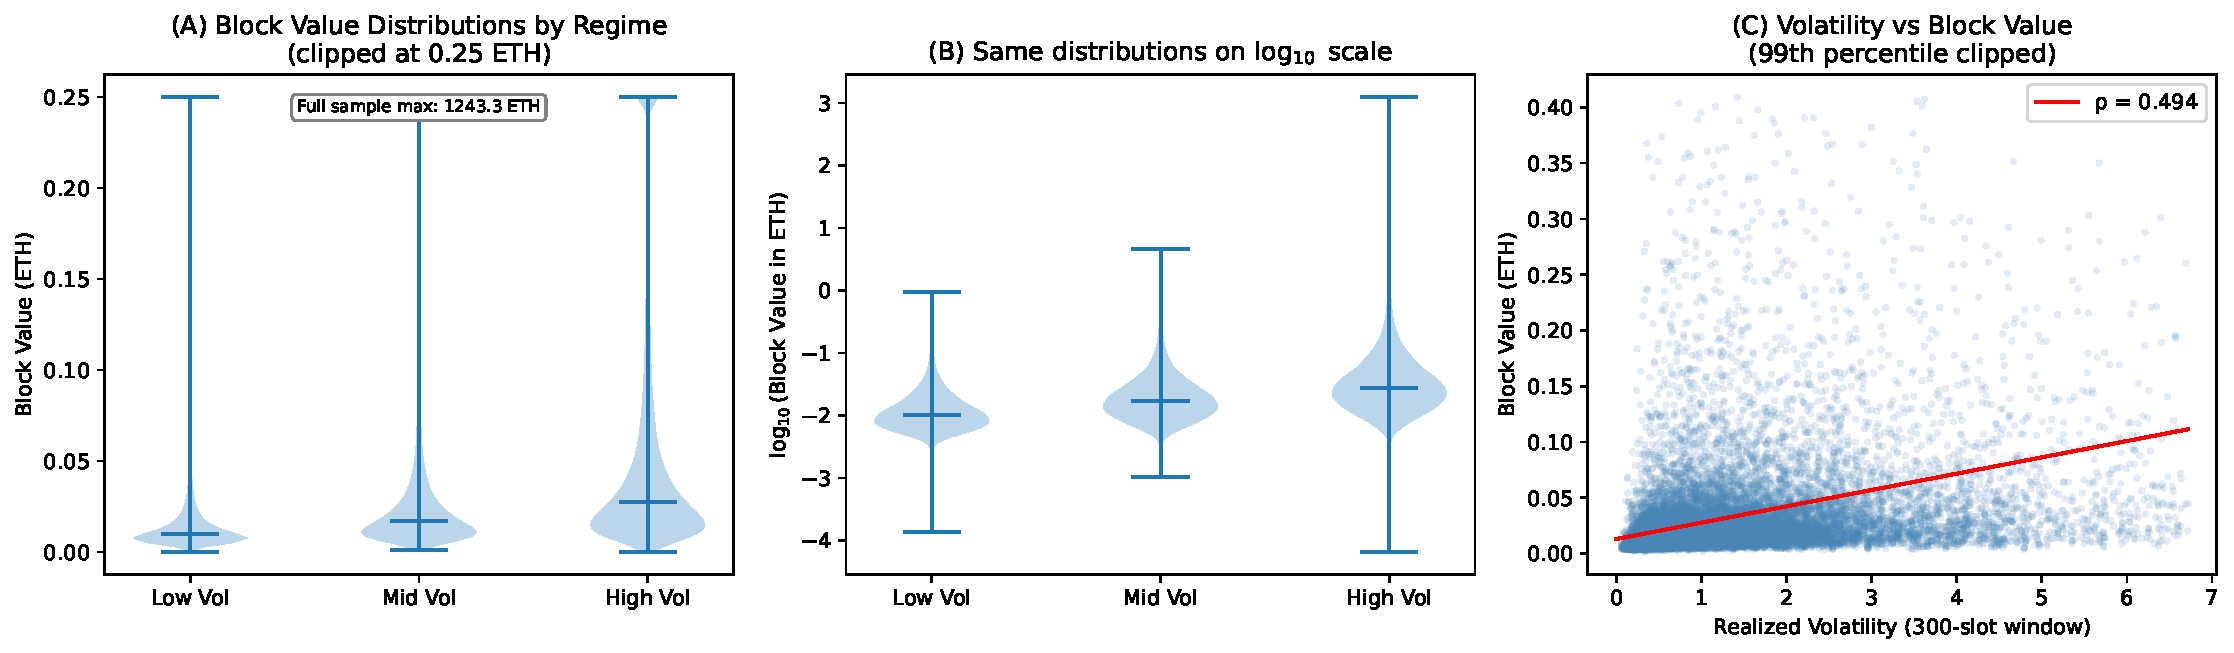
\includegraphics[width=\textwidth]{figures/fig_volatility_regimes.pdf}
\caption{(A) Block value distributions across volatility regimes, clipped at
0.25 ETH for readability. (B) Same distributions on a $\log_{10}$ scale
showing the full range. (C) Scatter of realized volatility against block value
with fitted linear trend. Full-sample Spearman $\rho = 0.494$
($p < 10^{-300}$); bootstrap mean $\hat\rho = 0.493$ (95\% CI: [0.477,
0.510], $B = 1{,}000$ samples).}
\label{fig:regimes}
\end{figure}

\begin{quote}
\textbf{Finding 1.} \textit{Block values are approximately 7.0$\times$ higher
on average during high-volatility regimes relative to low-volatility regimes
($H = 266{,}905$, $\rho = 0.494$, $p < 10^{-300}$). The effect is
substantially stronger than estimates from shorter sample periods, reflecting
the inclusion of significant market stress events across the 20-month sample.}
\end{quote}

\subsection{GARCH Dynamics of MEV Block Values}
\label{sec:garch}

Table~\ref{tab:ljungbox} reports Ljung-Box test results on squared log returns.

\begin{table}[h]
\centering
\caption{Ljung-Box test for ARCH effects in squared log returns ($n = 1{,}271{,}078$)}
\label{tab:ljungbox}
\begin{tabular}{lrl}
\toprule
Lags & Q-statistic & $p$-value \\
\midrule
10 & 257,972.5 & $< 10^{-300}$ \\
20 & 268,977.5 & $< 10^{-300}$ \\
50 & 280,427.9 & $< 10^{-300}$ \\
\bottomrule
\end{tabular}
\end{table}

Table~\ref{tab:garch} presents the GARCH(1,1) parameter estimates. The
estimated volatility persistence is $\hat\alpha + \hat\beta = 0.100 + 0.880 =
0.980$, indicating extremely high but non-unit-root volatility persistence.

\begin{table}[!htbp]
\centering
\caption{GARCH(1,1) parameter estimates with Student's $t$ errors, full 20-month sample}
\label{tab:garch}
\begin{tabular}{lrrrl}
\toprule
Parameter & Estimate & Std Error & $t$-stat & $p$-value \\
\midrule
$\mu$ (mean) & $-5.59 \times 10^{-6}$ & 0.00117 & $-0.00$ & 0.996 \\
$\omega$ (constant) & 2.5788 & 0.00476 & 541.4 & $< 0.001$ \\
$\alpha$ (ARCH) & 0.1000 & 0.000662 & 151.0 & $< 0.001$ \\
$\beta$ (GARCH) & 0.8800 & 0.000183 & 4797.7 & $< 0.001$ \\
$\nu$ (d.o.f.) & 4.0053 & 0.00152 & 2643.6 & $< 0.001$ \\
\bottomrule
\end{tabular}

\smallskip
\footnotesize $\hat\alpha + \hat\beta = 0.980$; AIC $= 7{,}067{,}110$; $n = 1{,}271{,}078$; converged
\end{table}

\bigskip

\begin{table}[!htbp]
\centering
\caption{GARCH robustness checks: volatility persistence ($\hat\alpha + \hat\beta$)}
\label{tab:robustness}
\begin{tabular}{llrl}
\toprule
Specification & Sample & Persistence & Note \\
\midrule
GARCH(1,1) & Full 20-month & 0.9800 & Stable \\
GARCH(1,1), winsorized 1\% & Full 20-month & 0.9800 & Stable \\
GARCH(1,1) & Subperiods & -- & Non-convergent \\
\bottomrule
\end{tabular}

\smallskip
\footnotesize Subperiod GARCH does not converge reliably due to the mixture-like distribution of $\log(1+v_t)$ returns at sub-annual horizons. The full-sample estimate is the most reliable characterisation.
\end{table}

\begin{figure}[!htbp]
\centering
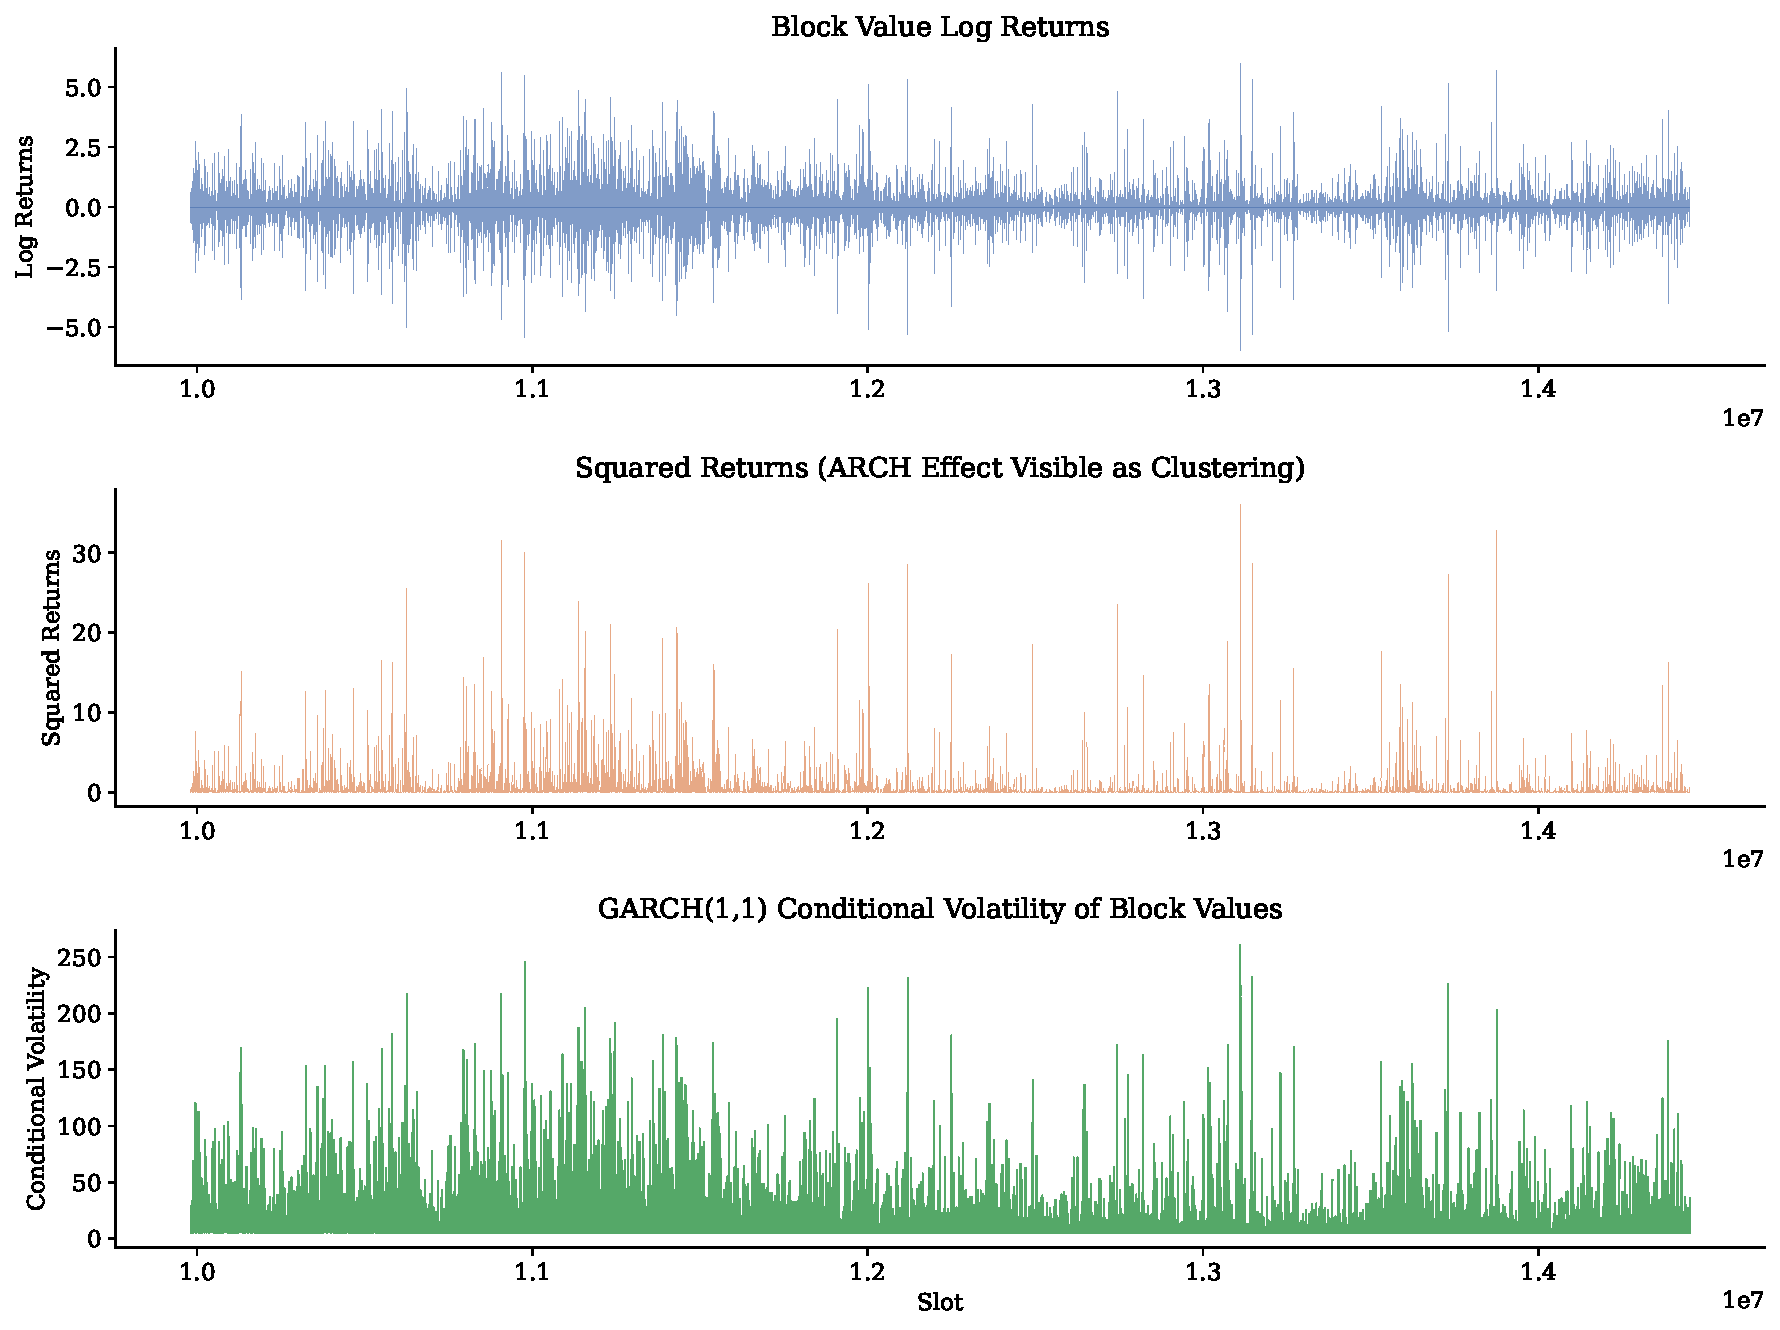
\includegraphics[width=\textwidth]{figures/fig_garch_clustering.pdf}
\caption{Top: Log returns of block values across 1,271,078 slots. Middle:
Squared returns, illustrating ARCH-type volatility clustering. Bottom:
GARCH(1,1) conditional volatility estimate $\hat\sigma_t$.}
\label{fig:garch}
\end{figure}

\begin{quote}
\textbf{Finding 2.} \textit{MEV block value log returns exhibit highly
persistent volatility dynamics ($\hat\alpha + \hat\beta = 0.980$) with
very heavy tails ($\hat\nu = 4.005$), confirmed across GARCH(1,1) and
winsorised specifications. A persistence of 0.980 implies that volatility
shocks retain approximately 82\% of their impact after ten periods.
Subperiod GARCH estimation is not reliable for this series due to the
non-standard distribution of $\log(1+v_t)$ returns at sub-annual horizons.}
\end{quote}

\subsection{Builder Market Concentration}
\label{sec:concentration}

Figure~\ref{fig:hhi} displays the weekly HHI and Gini coefficient over the full
20-month sample. The HHI began at approximately 2,100 in September 2024 and
declined sharply to approximately 800--900 by early 2025. A secondary period of
elevated concentration occurred in mid-2025 (HHI briefly reaching approximately
1,500), followed by a return to the unconcentrated range of 600--1,000.

\begin{figure}[h]
\centering
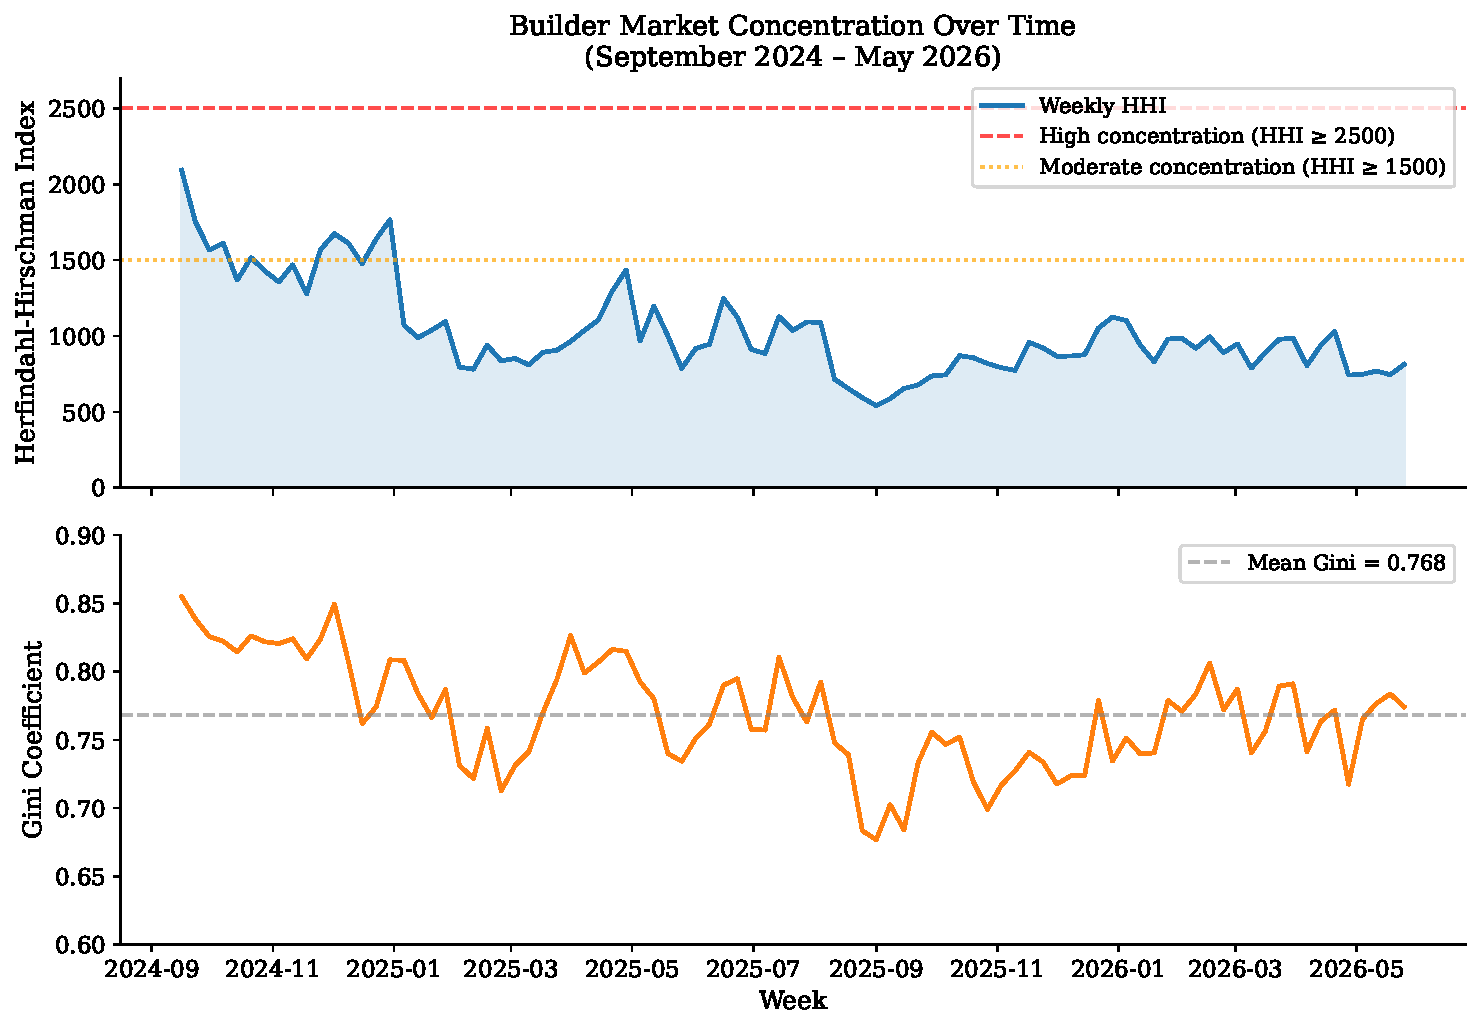
\includegraphics[width=\textwidth]{figures/fig_hhi_over_time.pdf}
\caption{Top: Weekly HHI of builder block production (eq.~\ref{eq:hhi}).
Bottom: Weekly Gini coefficient (eq.~\ref{eq:gini}). The HHI shows significant
initial deconcentration followed by cyclical variation, while the Gini declines
gradually from approximately 0.85 to 0.77.}
\label{fig:hhi}
\end{figure}

\begin{figure}[h]
\centering
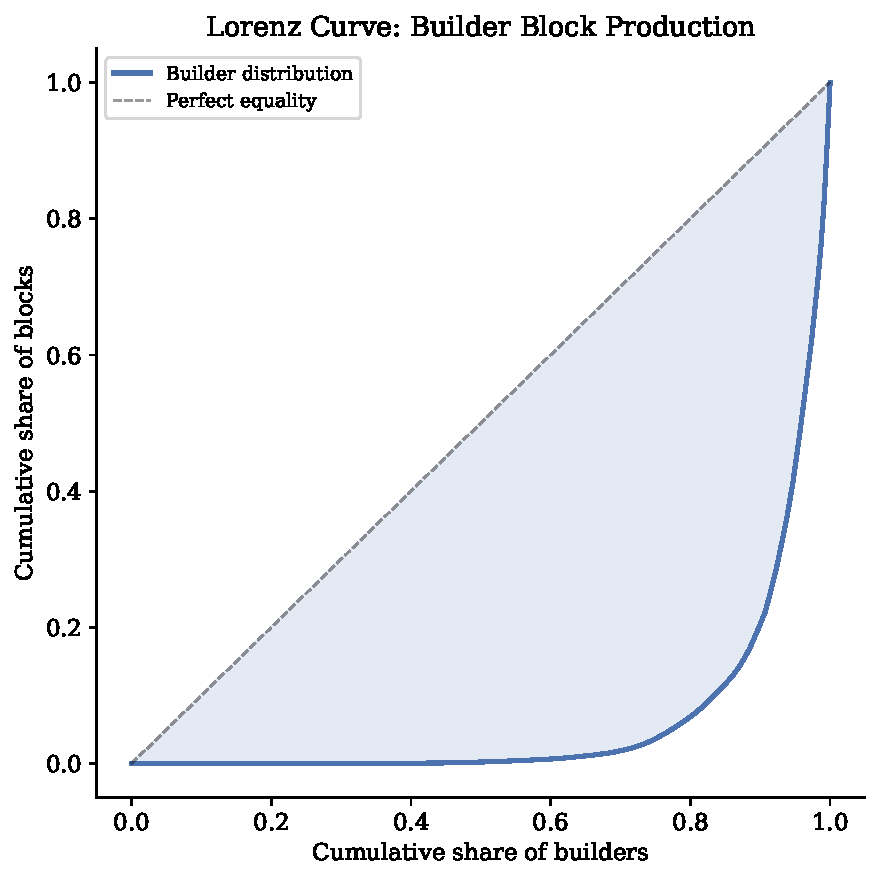
\includegraphics[width=0.7\textwidth]{figures/fig_lorenz_curve.pdf}
\caption{Lorenz curve of builder block production shares, full 20-month sample.
Pooled Gini $= 0.868$ across 227 builders: the bottom 50\% of builders account
for approximately 0.2\% of delivered blocks. The pooled full-sample Gini exceeds
the weekly-average Gini of 0.77 reported in Figure~\ref{fig:hhi} because
pooling over 20 months captures builders that were active only briefly.}
\label{fig:lorenz}
\end{figure}

\begin{quote}
\textbf{Finding 3.} \textit{Builder HHI declined from approximately 2,100 in
September 2024 to a stable unconcentrated range of 600--1,000, with a secondary
concentration episode in mid-2025 (HHI $\approx 1{,}500$). The Gini coefficient
declined from 0.85 to a long-run mean of 0.77.}
\end{quote}

\subsection{Temporal Patterns in MEV Activity}
\label{sec:temporal}

Figure~\ref{fig:temporal} displays mean block values by hour of day (UTC) and
day of week. The Kruskal-Wallis test rejects equal distributions across hours
($H = 65{,}875$, $df = 23$, $p < 10^{-300}$) and across days of the week
($H = 33{,}590$, $df = 6$, $p < 10^{-300}$). Block values are highest on
Monday (mean 0.086 ETH) and lowest on Saturday (0.031 ETH). The intraday
pattern is clearest in medians: median block value rises from approximately
0.012--0.013 ETH during 03:00--05:00 UTC to 0.020--0.024 ETH during
13:00--17:00 UTC, consistent with elevated activity during US trading hours.
Hourly means are dominated by a small number of extreme blocks (the 02:00 UTC
mean, for example, reflects a single outlier with hourly standard deviation
5.5 ETH) and should be read with that caveat.

\begin{figure}[h]
\centering
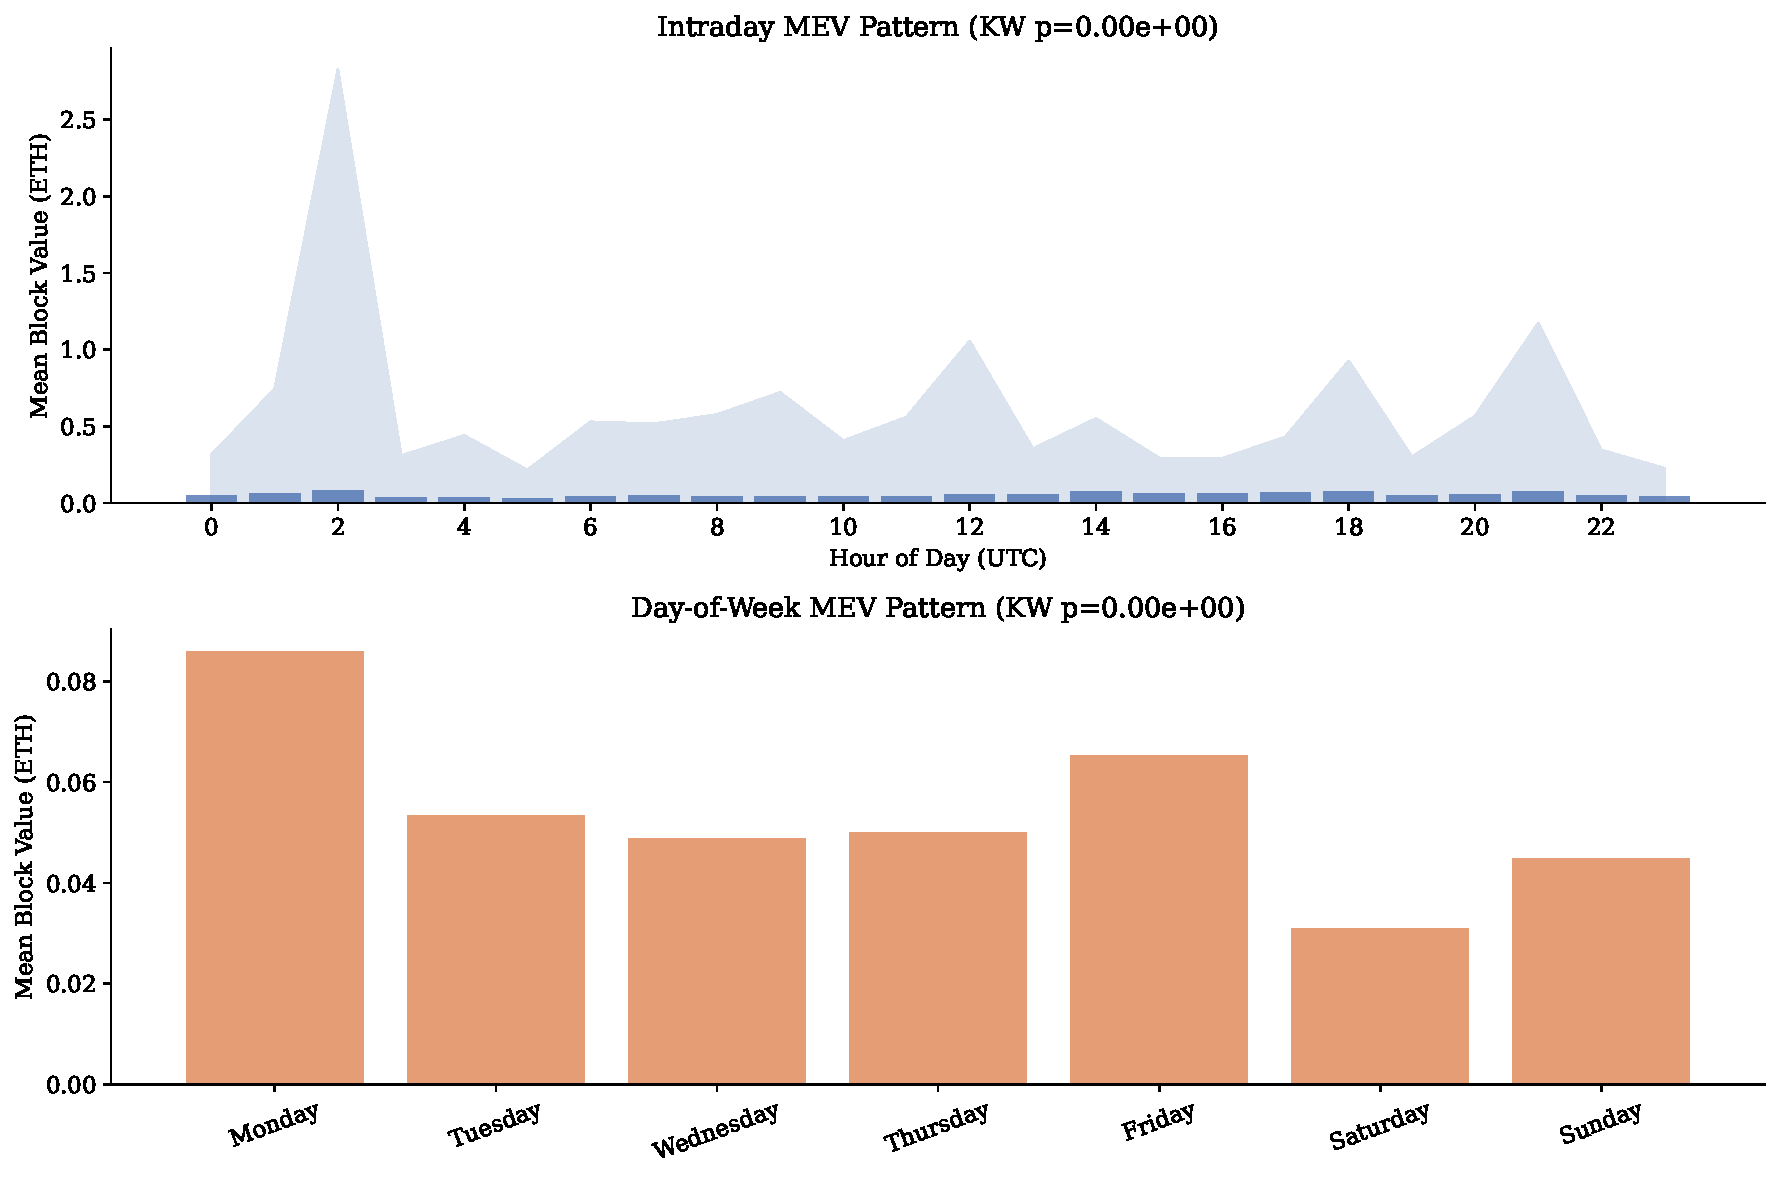
\includegraphics[width=\textwidth]{figures/fig_temporal_patterns.pdf}
\caption{Top: Mean block value by hour of day (UTC); isolated spikes reflect
individual extreme blocks rather than systematic patterns. Bottom: Mean block
value by day of week. Both panels show statistically significant variation
($p < 10^{-300}$).}
\label{fig:temporal}
\end{figure}

\begin{quote}
\textbf{Finding 4.} \textit{MEV block values exhibit statistically significant
intraday and day-of-week seasonality ($p < 10^{-300}$ in both cases). Median
block values peak during 13:00--17:00 UTC and are highest on Monday and
lowest on Saturday.}
\end{quote}

\subsection{Auction Microstructure}
\label{sec:auction}

\subsubsection{Overall Competitiveness}
\label{sec:overall_comp}

Table~\ref{tab:auction_summary} presents summary statistics for the auction
dataset across 1,220,100 matched slots. The PBS auction is highly competitive
at the median: builders submit a median of 132 bids per slot from 11 distinct
participants across 3 relays. Fewer than 0.001\% of slots exhibit a monopoly
configuration, indicating near-universal contestability.

\begin{table}[h]
\centering
\caption{Auction microstructure summary statistics, 1,220,100 matched slots,
September 2024 -- May 2026}
\label{tab:auction_summary}
\begin{tabular}{lrrrrr}
\toprule
Metric & Mean & Median & P10 & P90 & Max \\
\midrule
Bids per slot & 141.5 & 132 & 19 & 251 & 7{,}135 \\
Builders per slot & 11.5 & 11 & 7 & 17 & 37 \\
Relays per slot & 3.0 & 3 & 2 & 5 & 8 \\
Bid margin (\%) & 3.265 & 0.141 & 0.000 & 6.691 & 100.00 \\
Earliest bid (ms) & $-$7{,}916 & $-$8{,}090 & $-$11{,}018 & $-$3{,}898 & 0 \\
Latest bid (ms) & 2{,}187 & 2{,}058 & 629 & 3{,}647 & 22{,}082 \\
\bottomrule
\end{tabular}
\end{table}

The distribution of bid margins is highly right-skewed: the median of 0.141\%
implies near-perfect competition in typical slots, while the 90th-percentile
margin of 6.691\% indicates that one in ten slots exhibits materially reduced
competition. Figure~\ref{fig:auction_competitiveness} displays the full
distributions of bid counts, builder participation, and bid margins.

\begin{figure}[h]
\centering
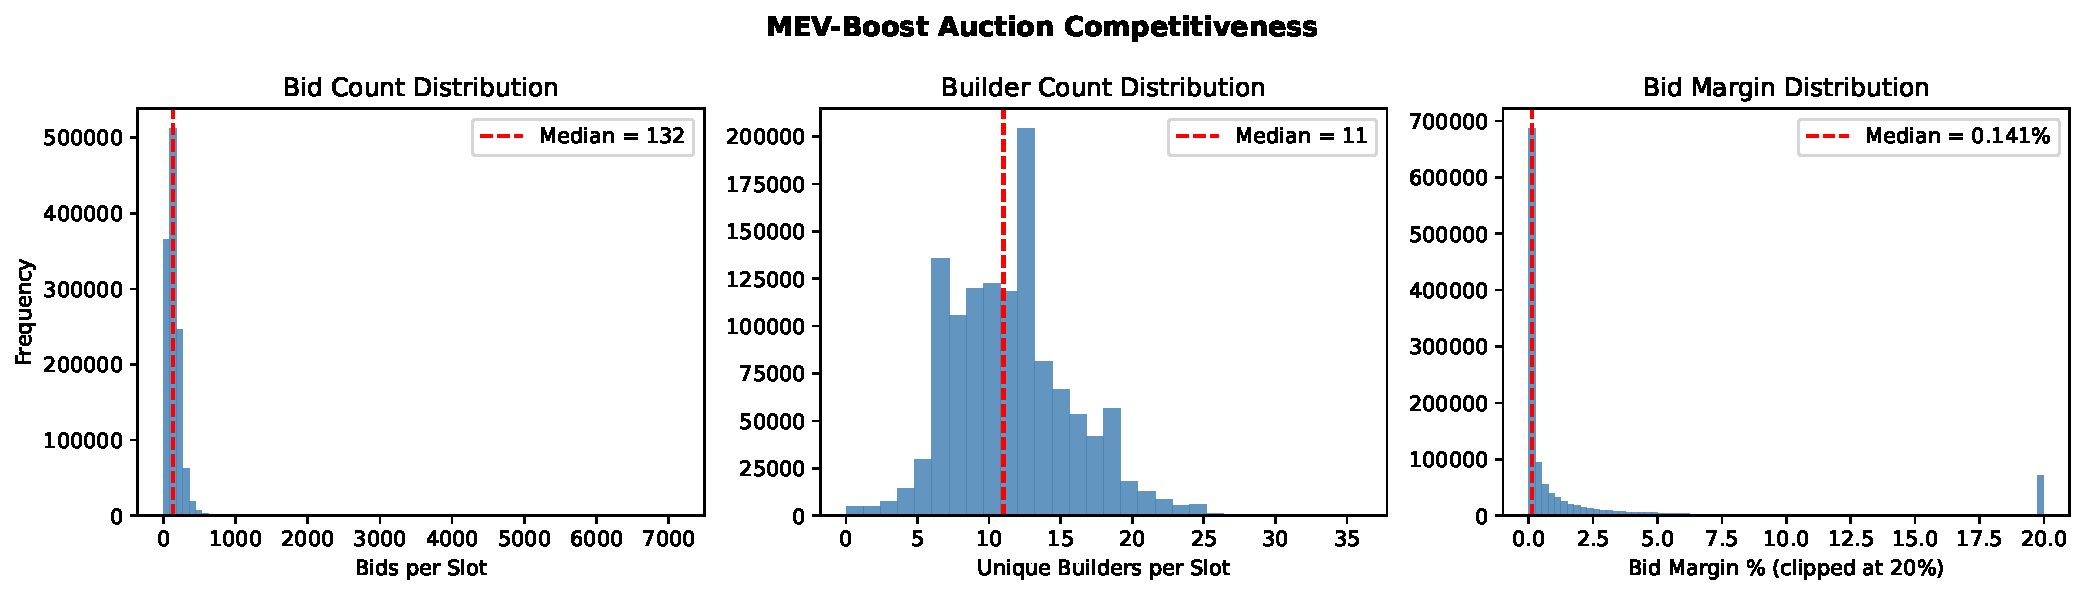
\includegraphics[width=\textwidth]{figures/fig_auction_competitiveness.pdf}
\caption{Distribution of auction competitiveness metrics across 1,220,100
matched slots. Left: bid count per slot (median 132). Centre: unique builders
per slot (median 11). Right: bid margin distribution, clipped at 20\% for
readability (median 0.141\%).}
\label{fig:auction_competitiveness}
\end{figure}

\subsubsection{Competitiveness Increases with Block Value}
\label{sec:comp_value}

Figure~\ref{fig:margin_vs_value} displays the relationship between block value
and bid margin. Bid margins decline monotonically as block value increases,
with median margins of 0.196\%, 0.144\%, and 0.110\% for low-, mid-, and
high-value terciles respectively. Spearman's rank correlation between block
value and bid margin is $\rho = -0.054$ ($p < 10^{-300}$, $n =
1{,}219{,}851$; bootstrap 95\% CI $[-0.075, -0.031]$, $B=1{,}000$). Builder
participation exhibits a stronger positive association with block value
($\rho = 0.286$, $p < 10^{-300}$; bootstrap 95\% CI $[0.265, 0.305]$):
high-value slots attract substantially more builders.

The compression of bid margins in high-value slots provides an auction-theoretic
mechanism underlying the volatility-value correlation documented in Finding~1:
in the slots where MEV opportunity is largest, proposers capture a larger share
of that value because competition drives bids toward the true block value.

\begin{figure}[h]
\centering
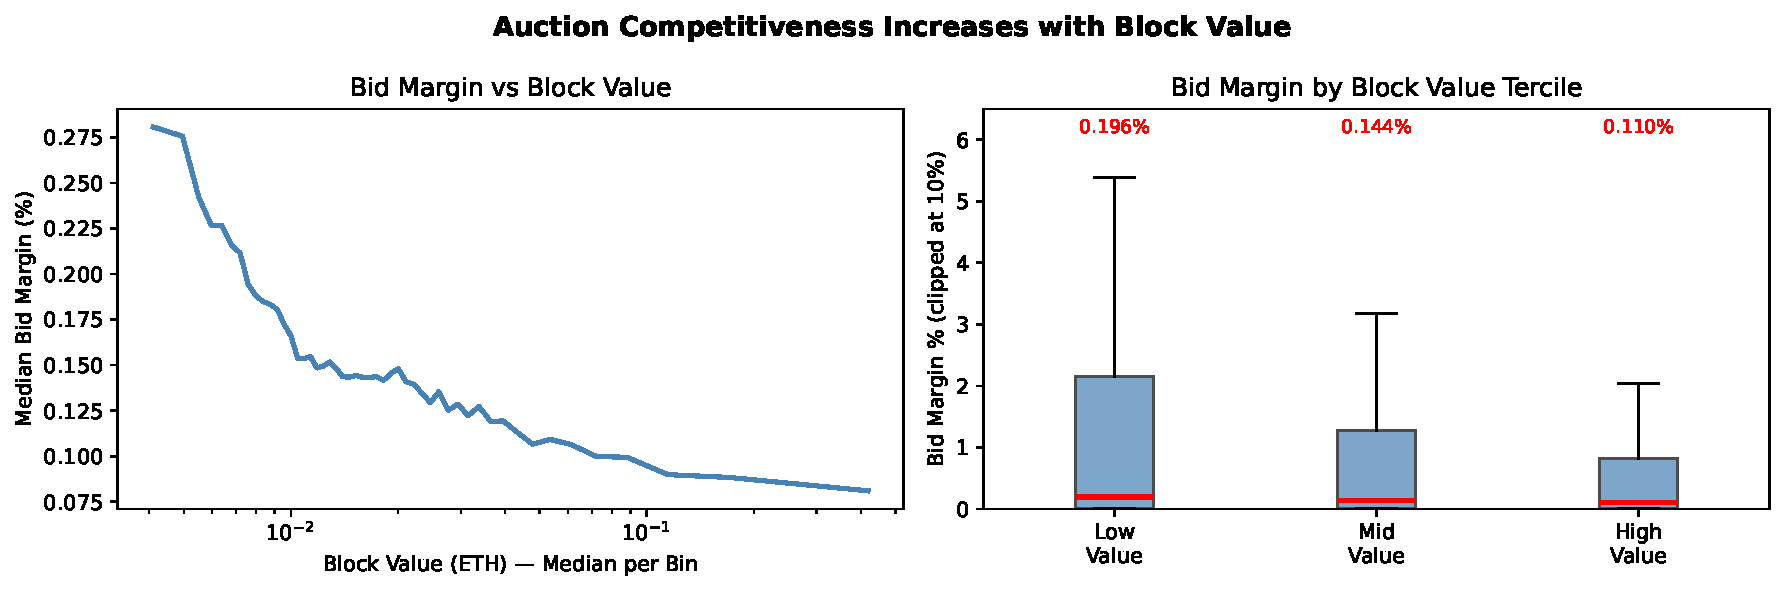
\includegraphics[width=\textwidth]{figures/fig_margin_vs_value_fixed.pdf}
\caption{Left: scatter of bid margin against block value (log scale) with
rolling median (red line). Right: bid margin distributions by block value
tercile (outliers removed; median annotated in red). Bid margins compress
monotonically with block value, consistent with intensified competition for
high-MEV slots.}
\label{fig:margin_vs_value}
\end{figure}

\begin{quote}
\textbf{Finding 5a.} \textit{Bid margins compress monotonically with block
value (0.196\%, 0.144\%, 0.110\% across low, mid, and high value terciles;
$\rho = -0.054$, $p < 10^{-300}$), and builder participation increases with
block value ($\rho = 0.286$, $p < 10^{-300}$). High-value slots are both more
competitive and more efficiently allocated.}
\end{quote}

\subsubsection{Bid Timing}
\label{sec:bid_timing_sec}

Figure~\ref{fig:bid_timing} displays the distribution of earliest and latest
bid arrival times. Builders begin submitting bids a median of 8,090\,ms before
slot start, indicating that bidding activity commences during the preceding
slot's window. Latest bid arrivals are concentrated around 2,058\,ms after slot
start, with 5.3\% of slots receiving bids more than 4,000\,ms after slot start.

\begin{figure}[h]
\centering
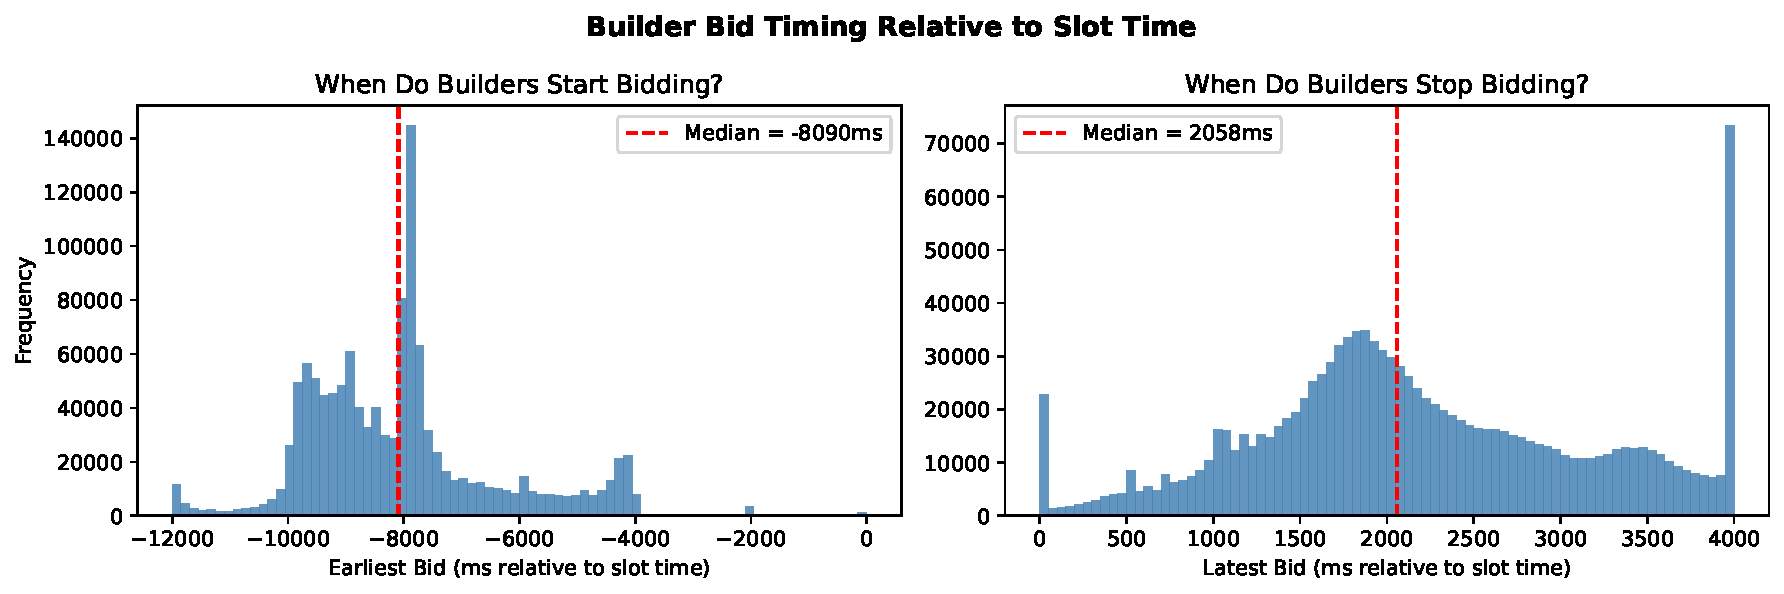
\includegraphics[width=\textwidth]{figures/fig_bid_timing.pdf}
\caption{Builder bid timing relative to slot start ($\tau = 0$), across
1,220,100 matched slots. Left: earliest bid arrival (median $-8{,}090$\,ms).
Right: latest bid arrival (median $+2{,}058$\,ms); 5.3\% of slots receive bids
after $+4{,}000$\,ms.}
\label{fig:bid_timing}
\end{figure}

Figure~\ref{fig:timing_by_value} shows that high-value slots attract later bids
($\rho = 0.146$, $p < 10^{-300}$; bootstrap 95\% CI $[0.125, 0.169]$) and more builders. Builders extend their
bidding window when the potential reward is larger, consistent with rational
cost-benefit behaviour.

\begin{figure}[h]
\centering
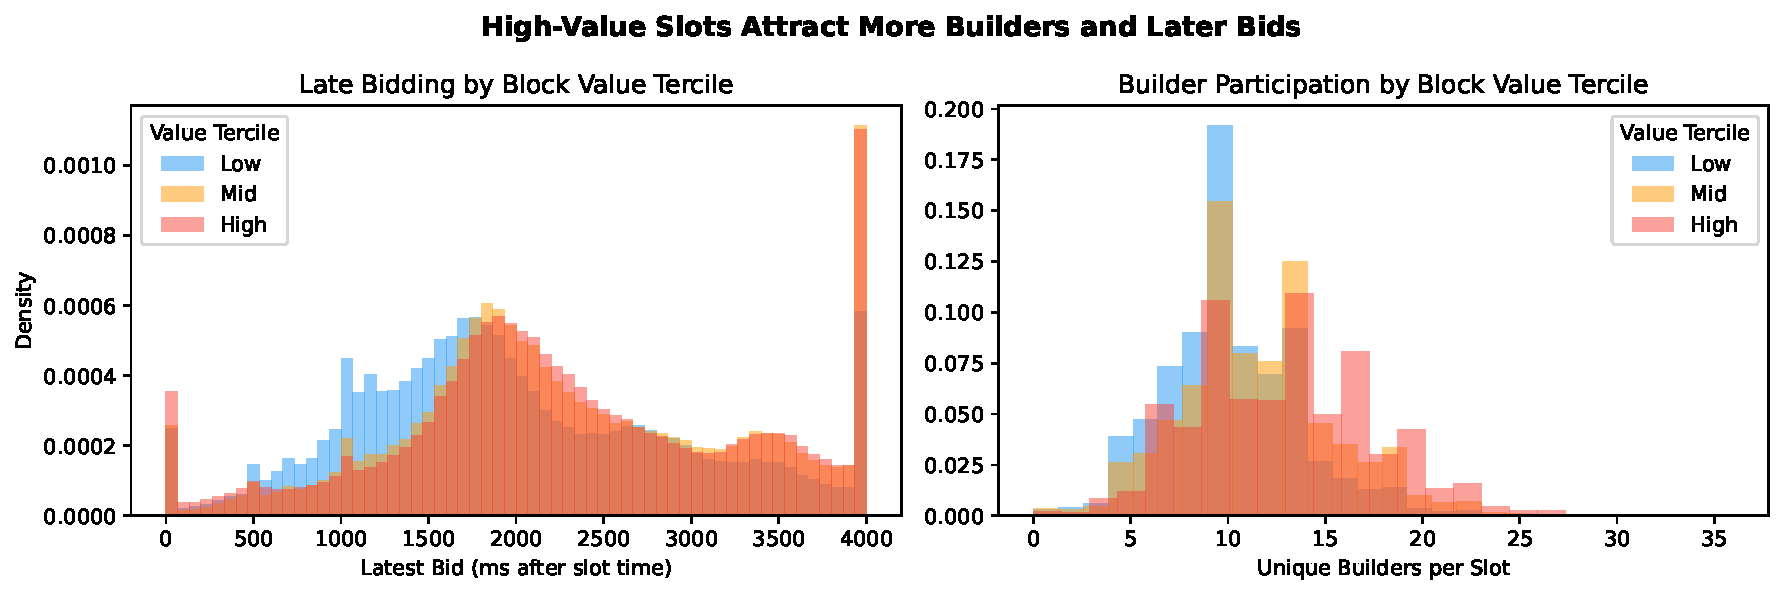
\includegraphics[width=\textwidth]{figures/fig_timing_by_value.pdf}
\caption{Left: distribution of latest bid arrival time by block value tercile.
High-value slots exhibit a rightward shift, indicating later bidding when
rewards are larger. Right: builder participation distributions by value
tercile.}
\label{fig:timing_by_value}
\end{figure}

\begin{quote}
\textbf{Finding 5b.} \textit{Builders begin bidding a median of 8,090\,ms
before slot start and continue until a median of 2,058\,ms after slot start.
High-value slots attract later bids ($\rho = 0.146$, $p < 10^{-300}$) and more
builders ($\rho = 0.286$, $p < 10^{-300}$), consistent with rational extension
of the bidding window in pursuit of higher expected payoffs.}
\end{quote}

\subsubsection{Temporal Evolution of Auction Competitiveness}
\label{sec:comp_evolution}

Figure~\ref{fig:competitiveness_timeseries} displays weekly medians of bid
margin, builder participation, and bid count over the full 20-month sample.
None of the three series exhibits the monotone ``deepening'' that a naive
maturation narrative would predict. Median builder participation
\emph{declined} on net, from approximately 17 builders per slot in late 2024
to approximately 9--11 by 2026. Median bid counts are cyclical without a
clear trend, fluctuating between roughly 75 and 225 per slot around a
full-sample median of 132. Median bid margins show no sustained compression:
they oscillate between approximately 0.05\% and 0.3\% through 2025 and are,
if anything, elevated (0.2--0.5\%) during December 2025 -- March 2026.
Monthly matched-slot counts also jump roughly five-fold during January--April
2025 relative to adjacent months, reflecting uneven bid-archive coverage
rather than a change in auction activity; the weekly medians are robust to
this because they condition on matched slots, but level comparisons across
that boundary should be made with care.

\begin{figure}[h]
\centering
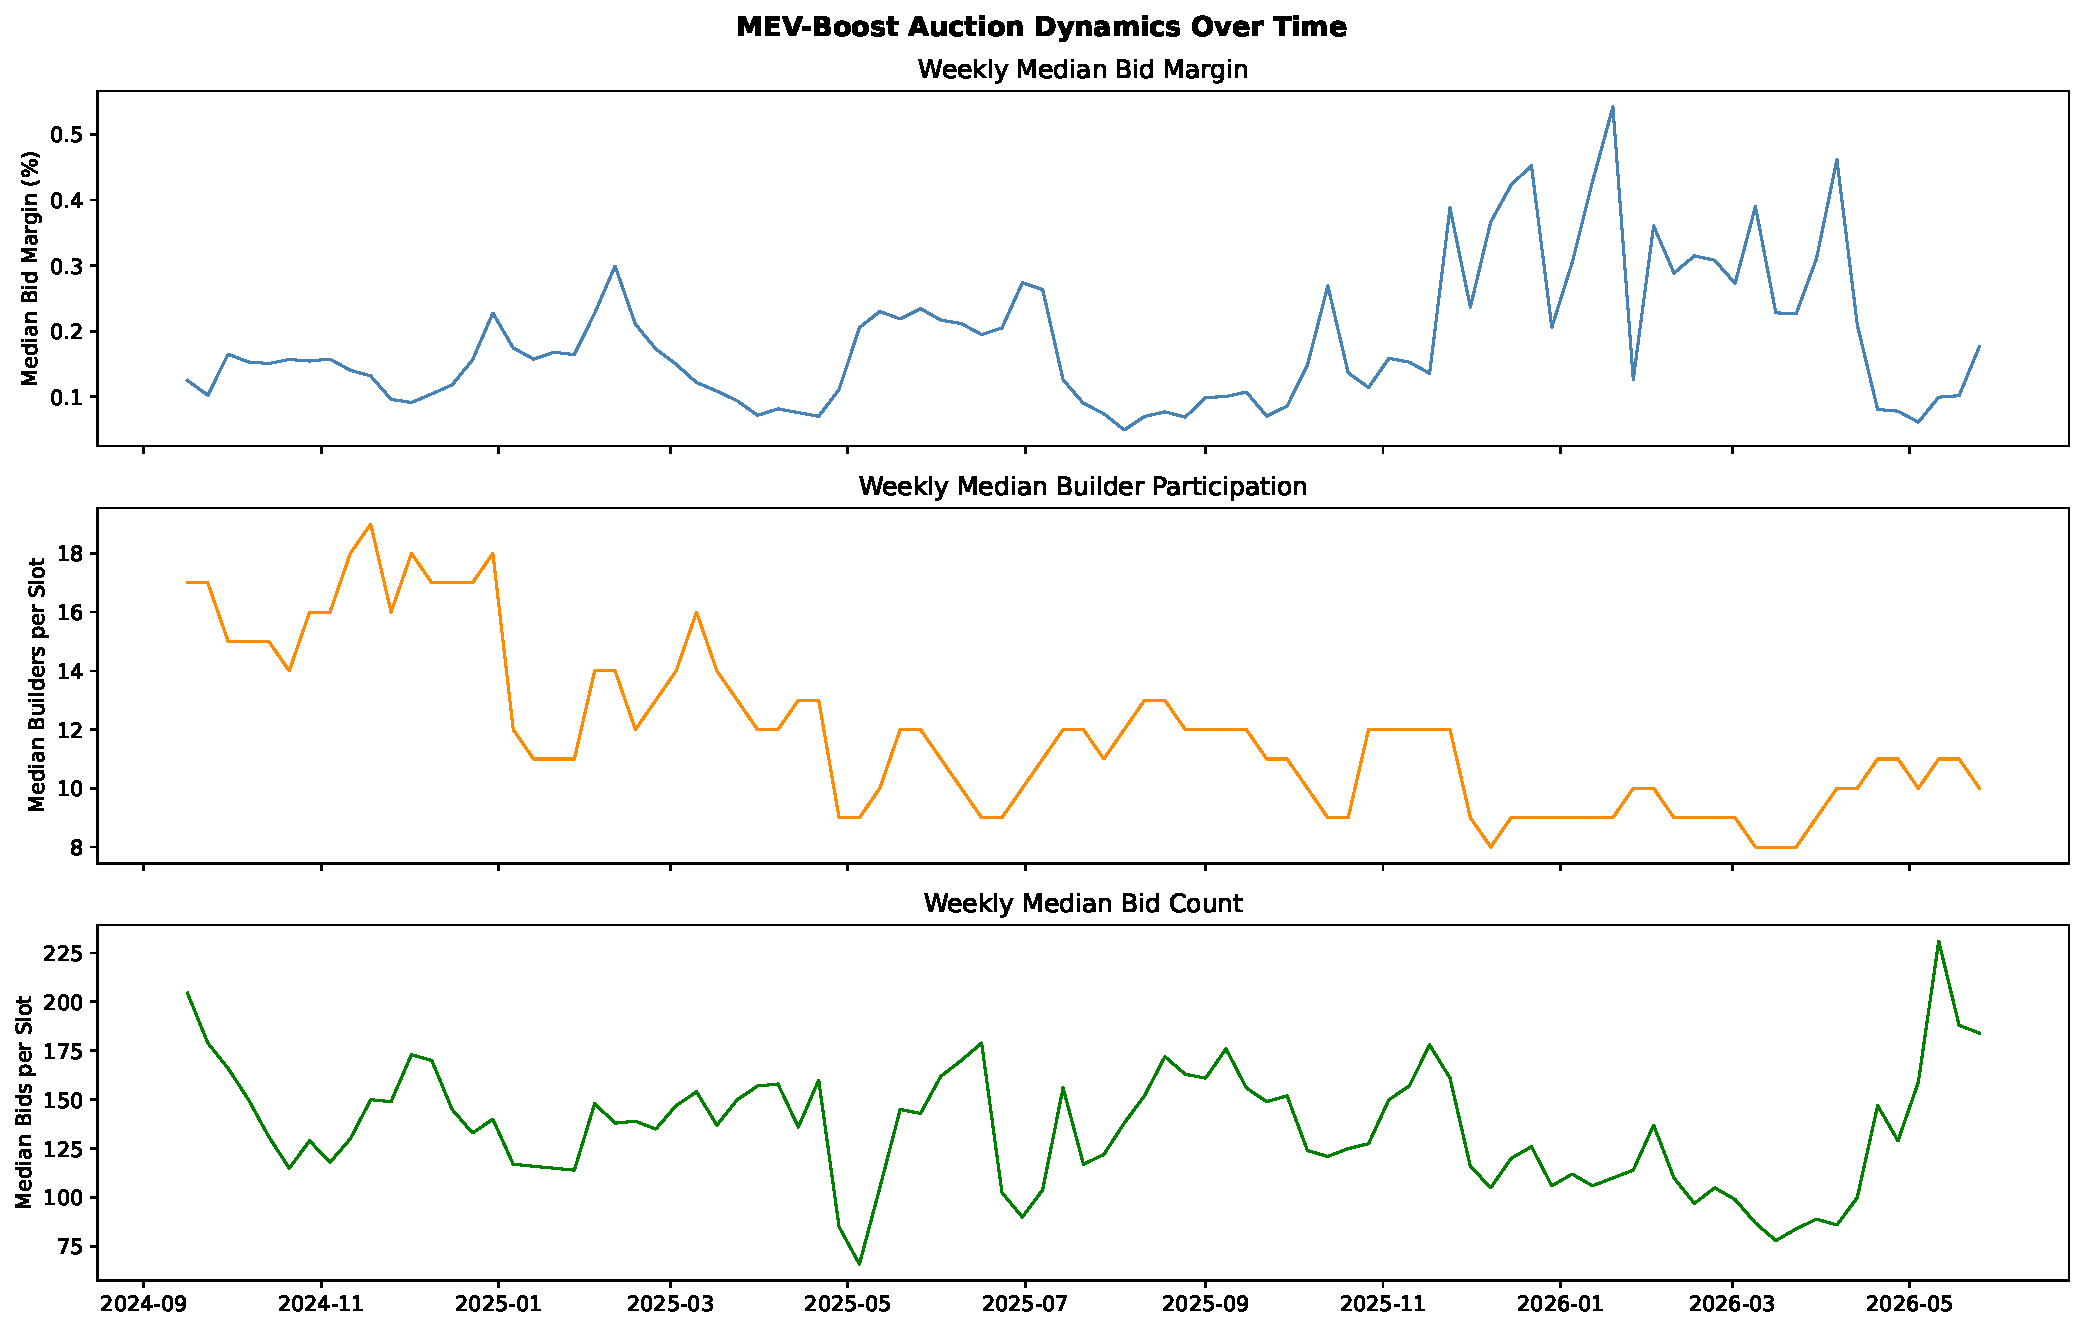
\includegraphics[width=\textwidth]{figures/fig_competitiveness_timeseries.pdf}
\caption{Weekly medians of auction competitiveness metrics, September 2024 --
May 2026. Top: median bid margin (no sustained trend; elevated in late
2025 -- early 2026). Middle: median builder participation (declining from
approximately 17 to 9--11 per slot). Bottom: median bid count (cyclical,
no clear trend).}
\label{fig:competitiveness_timeseries}
\end{figure}

Read against the HHI deconcentration documented in
Section~\ref{sec:concentration}, this is a picture of consolidation rather
than entry: the number of builders actively bidding per slot fell by roughly
40\% while the distribution of \emph{delivered} blocks among the remaining
builders became more even. Fewer, more evenly matched competitors can produce
both a lower HHI and stable margins, which is what the data show.

Table~\ref{tab:margin_reg} formalises these bivariate relationships in a
multivariate setting, regressing bid margin jointly on log block value,
builder count, relay count, hour of day, and day of week. All five
predictors remain statistically significant ($p < 0.001$) with the expected
signs after controlling for the others: a one-unit increase in log block
value is associated with a 0.76 percentage point decline in margin, each
additional builder with a 0.16 percentage point decline, and each additional
relay with a 0.72 percentage point decline --- relay participation has the
largest independent effect on margin compression among the three
auction-structure variables. The model explains a modest but
significant share of margin variance ($R^2 = 0.020$), consistent with bid
margins being driven by many factors beyond the five auction-structure
variables considered here, including builder-specific cost structures and
idiosyncratic orderflow access documented in Section~\ref{sec:builder_strat}.

\begin{quote}
\textbf{Finding 5c.} \textit{The PBS auction has consolidated rather than
deepened: median builder participation declined from approximately 17 to
9--11 builders per slot over the sample, while median bid counts (75--225)
and bid margins (0.05--0.5\%) fluctuate cyclically without a sustained
trend. Combined with the HHI deconcentration in delivered blocks, this
indicates a smaller but more evenly matched set of active builders.}
\end{quote}



%------------------------------------------------------------------
% SECTION 5.6 — Extended Auction Analysis
%------------------------------------------------------------------
\subsection{Extended Auction Analysis}
\label{sec:extended_auction}

\subsubsection{ETH Price Decomposition}
\label{sec:eth_decomp_sec}

A key limitation of prior PBS analyses is the conflation of ETH price
movements with MEV-specific dynamics. We address this directly using 15,302
hourly ETH/USD price observations from Coinbase (September 2024--May 2026),
matched to delivered payload slots by hour.

Of the 1,271,079 delivered payload slots, 1,218,882 (95.9\%) are matched to
an hourly ETH price observation; the unmatched remainder corresponds to hours
for which no Coinbase price bar was retrieved. We regress log block value (ETH) on log ETH
price and find:

\begin{equation}
\log(v_t) = -4.172 + 0.027 \cdot \log(P_t^{\text{ETH}}) + \varepsilon_t,
\quad R^2 = 0.0001
\label{eq:eth_decomp}
\end{equation}

where $P_t^{\text{ETH}}$ denotes the hourly ETH/USD closing price. ETH price
explains essentially zero variance in block value when both are denominated in
ETH (Spearman $\rho = 0.050$, $p < 10^{-300}$). However, when block value is
converted to USD, the association strengthens substantially (Spearman $\rho =
0.359$, $p < 10^{-300}$), reflecting the mechanical co-movement of any
ETH-denominated quantity with its USD equivalent.

These results establish that MEV block value in ETH is driven by on-chain
activity---transaction ordering opportunities, arbitrage spreads, and
liquidation events---rather than by ETH price movements. The volatility regime
effects documented in Finding~1 (7.0$\times$ block value increase in
high-volatility periods) therefore reflect genuine variation in on-chain MEV
opportunity, not a repricing artifact of ETH/USD fluctuations.

\begin{figure}[h]
\centering
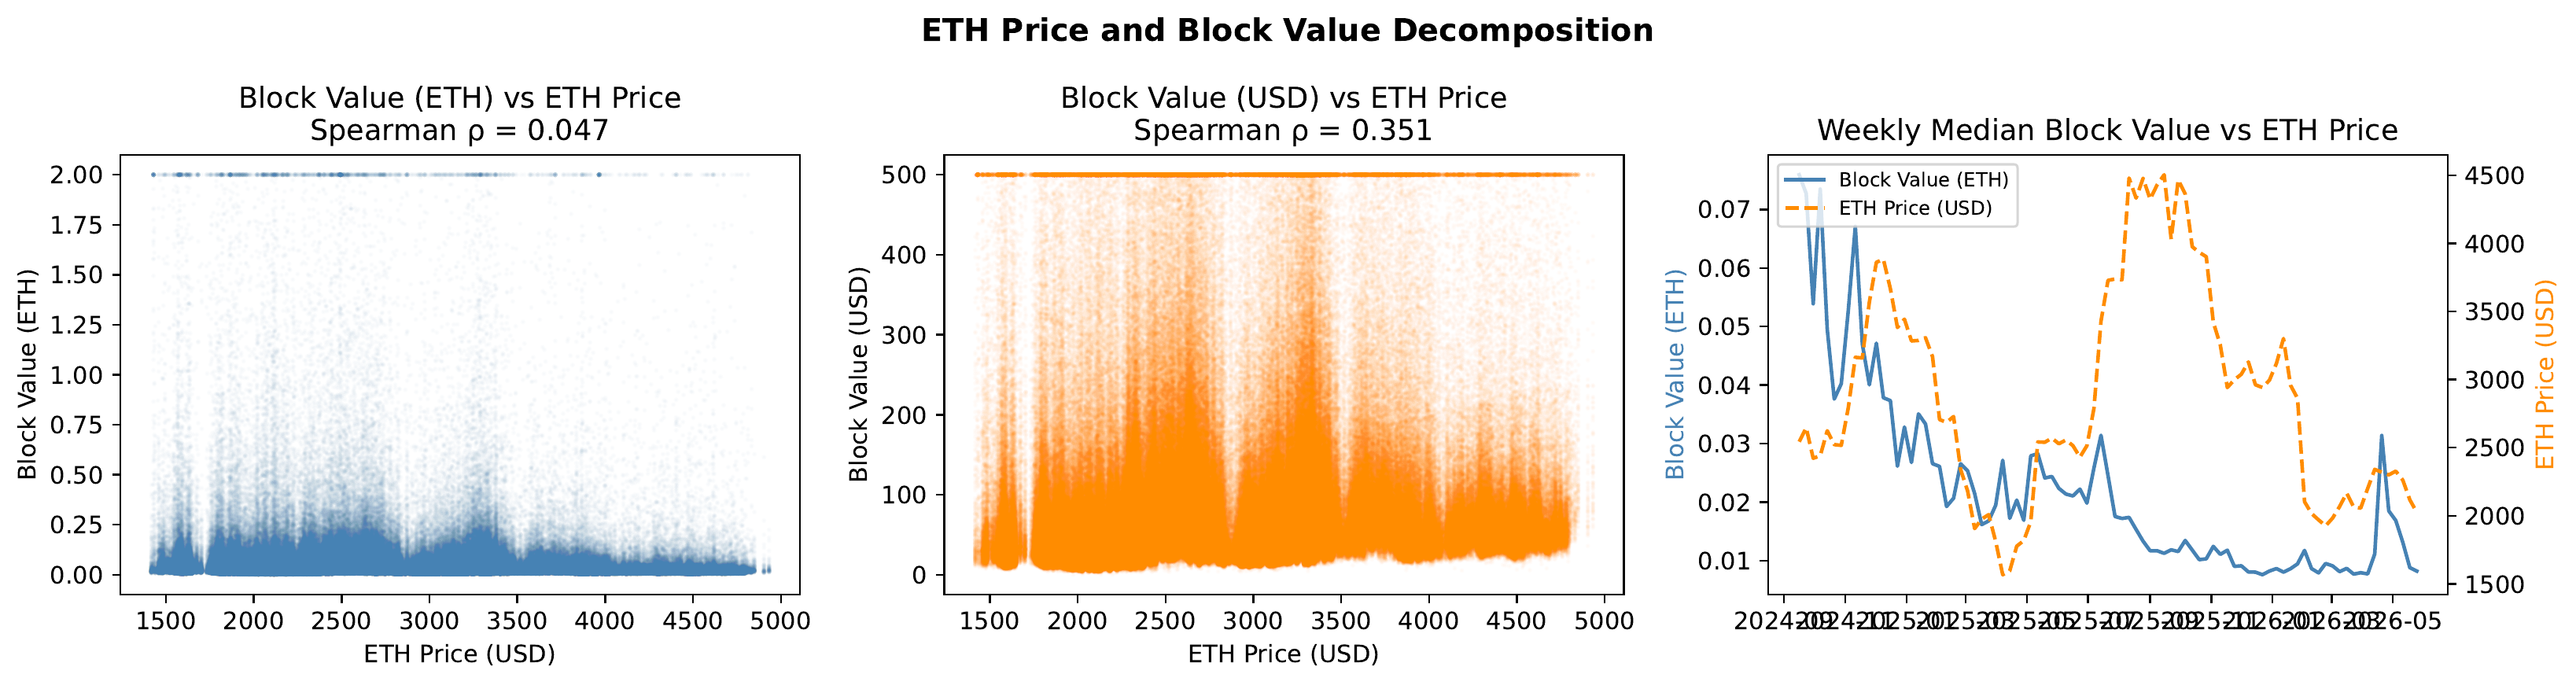
\includegraphics[width=\textwidth]{figures/fig_eth_decomposition.png}
\caption{ETH price and block value decomposition. Left: block value in ETH vs
ETH price (Spearman $\rho = 0.050$); MEV opportunity is orthogonal to ETH
price in ETH terms. Centre: block value in USD vs ETH price ($\rho = 0.359$),
reflecting mechanical USD conversion. Right: weekly median block value (ETH,
blue) and ETH price (USD, orange) co-plotted, confirming the visual
decoupling in ETH terms.}
\label{fig:eth_decomp}
\end{figure}

\begin{quote}
\textbf{Finding 6.} \textit{ETH price explains essentially zero variance in
block value when denominated in ETH ($R^2 = 0.0001$, Spearman $\rho = 0.050$),
but explains meaningful variance in USD terms ($\rho = 0.359$). MEV block
value is driven by on-chain activity, not ETH price movements. The 7.0$\times$
volatility regime effect documented in Finding~1 reflects genuine variation in
MEV opportunity.}
\end{quote}


\begin{table}[h]
\centering
\caption{OLS regression of bid margin on auction structure variables
($n = 1{,}219{,}851$, HC0 robust standard errors)}
\label{tab:margin_reg}
\begin{tabular}{lrrrr}
\toprule
Variable & Coefficient & Robust SE & $t$-stat & $p$-value \\
\midrule
Intercept & 3.7968 & 0.0620 & 61.24 & $<$0.001 \\
$\log(\text{Block Value})$ & $-$0.7576$^{***}$ & 0.0092 & $-$82.62 & $<$0.001 \\
N Builders & $-$0.1564$^{***}$ & 0.0024 & $-$66.24 & $<$0.001 \\
N Relays & $-$0.7190$^{***}$ & 0.0078 & $-$92.56 & $<$0.001 \\
Hour of Day & 0.0080$^{***}$ & 0.0013 & 6.01 & $<$0.001 \\
Day of Week & 0.0119$^{*}$ & 0.0047 & 2.51 & 0.012 \\
\bottomrule
\end{tabular}
\vspace{0.5em}
\footnotesize $R^2 = 0.020$. $^{***}p < 0.001$, $^{*}p < 0.05$. Dependent variable: bid margin (\%).
Each additional builder reduces the margin by 0.16 percentage points; each additional
relay reduces it by 0.72 percentage points, holding other variables constant.
\end{table}

\begin{figure}[h]
\centering
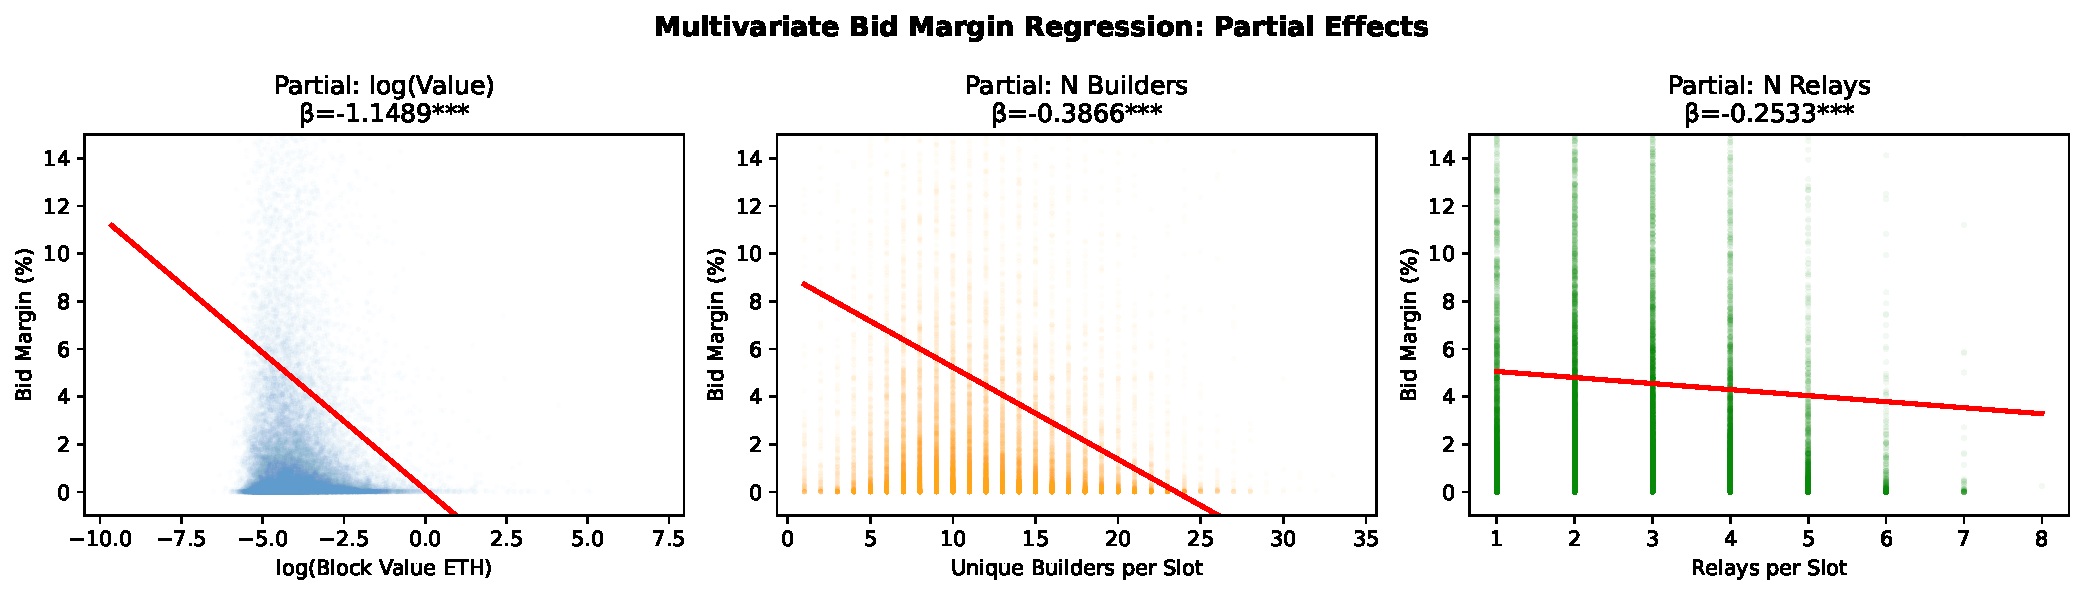
\includegraphics[width=\textwidth]{figures/fig_margin_regression.pdf}
\caption{Partial regression plots for the three main auction structure variables.
Red lines show OLS fitted values at mean levels of all other regressors.
All three variables are statistically significant ($p < 0.001$) with the
expected negative sign, confirming that block value, builder participation,
and relay participation independently reduce bid margins.}
\label{fig:margin_reg}
\end{figure}


\subsubsection{Isolating MEV-Specific Volatility Persistence}
\label{sec:mev_specific}

To formally confirm that the GARCH persistence documented in Finding~2 is
driven by MEV-specific dynamics rather than ETH price movements, we regress
the block-value log return series on the contemporaneous ETH price log return
and re-estimate GARCH(1,1) on the residual. The regression yields
$R^2 \approx 0.0000$ ($n=1{,}269{,}860$), confirming that ETH price returns
explain essentially none of the variance in block-value returns at the
slot level, consistent with Finding~6.

GARCH(1,1) estimated on this MEV-specific residual series yields
$\hat\alpha + \hat\beta = 0.980$ ($\hat\nu = 4.005$), numerically identical
to the full block-value return series. This confirms that the high
volatility persistence documented in Finding~2 is a property of MEV
dynamics in isolation, not an artifact of correlated ETH price movements.
The PBS auction's volatility clustering is therefore a genuinely on-chain
phenomenon, reinforcing the interpretation in Section~\ref{sec:eth_decomp_sec}
that MEV
extraction opportunity is fundamentally driven by transaction-level
activity rather than asset price dynamics.

\subsubsection{Relay Participation as a Determinant of Auction Depth}
\label{sec:relay_depth}

We examine whether the number of relays through which bids are received per
slot predicts auction competitiveness. Table~\ref{tab:relay_margin} presents
median bid margins by relay count.

\begin{table}[h]
\centering
\caption{Bid margin by relay count per slot}
\label{tab:relay_margin}
\begin{tabular}{lrr}
\toprule
Relays per Slot & Median Bid Margin (\%) & Slot Count \\
\midrule
1 & 0.217 & 213,316 \\
2 & 0.143 & 401,220 \\
3 & 0.124 & 350,993 \\
4 & 0.124 & 195,353 \\
5 & 0.109 & 49,090 \\
6 & 0.084 & 8,714 \\
7 & 0.066 & 1,112 \\
\bottomrule
\end{tabular}
\end{table}

Bid margins decline monotonically from 0.217\% in single-relay slots to
0.066\% in 7-relay slots, a 3.3$\times$ compression. Spearman's rank
correlation confirms the relationship (excluding the two sparse extreme
categories): $\rho = -0.057$, $p < 10^{-300}$. While the effect size is
modest, the monotone pattern across seven relay-count categories and the
statistical significance across 1.2M observations establish relay
participation as a structural determinant of auction depth. Slots reaching
more relays expose builders to wider competition, driving margins lower.

\begin{figure}[h]
\centering
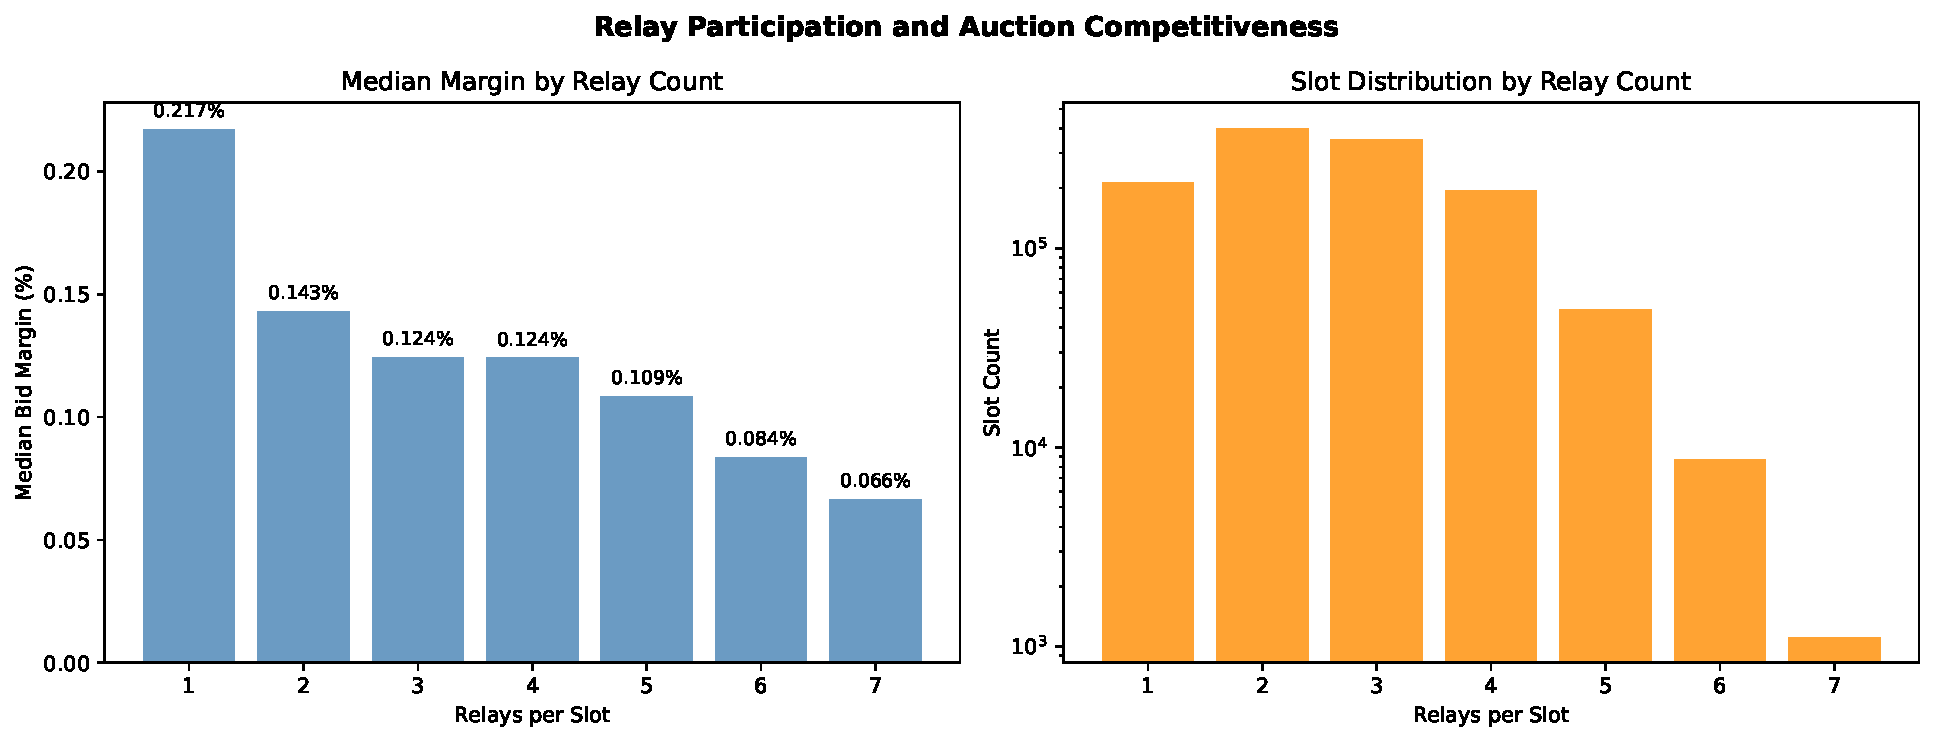
\includegraphics[width=\textwidth]{figures/fig_relay_analysis.pdf}
\caption{Left: median bid margin by relay count per slot. Margins decline
monotonically from 0.217\% (1 relay) to 0.066\% (7 relays). Right: slot
distribution by relay count; 2--3 relays account for the majority of slots.}
\label{fig:relay_analysis}
\end{figure}

\begin{quote}
\textbf{Finding 7.} \textit{Relay participation is a structural determinant
of auction competitiveness: bid margins decline monotonically from 0.217\%
in single-relay slots to 0.066\% in 7-relay slots ($\rho = -0.057$,
$p < 10^{-300}$; bootstrap 95\% CI $[-0.079, -0.035]$, $B=1{,}000$). Broader
relay participation exposes builders to wider competition, compressing
margins by up to 3.3$\times$.}
\end{quote}

\subsubsection{Builder Strategy Heterogeneity}
\label{sec:builder_strat}

Analysis of 5,130,040 bid observations across 144 builders in a Q1 2025
weekly sample initially suggested three bidding clusters, including a
small group of builders whose bids arrived after slot start with
markedly higher median values. To test whether this reflected genuine
builder strategy or an artifact of relay-side data collection, we
reprocessed the complete (non-sampled) Q1 2025 bid archive --- 90 daily
files, 86,805,657 bid observations --- and compared bid timing for the
same builders across different relays.

The results show that bid timing is overwhelmingly a property of the
\emph{relay}, not the builder. Pooling all builders, median bid timing
ranges from $-4{,}913$\,ms (securerpc) to $+2{,}497$\,ms (Titan) depending
on relay, a spread of nearly 7.4 seconds driven entirely by
relay-specific data collection and reporting characteristics; ultrasound
alone contributes 96.3\% of all observations with a median of $-710$\,ms,
while bloxroost's two endpoints report medians of $+2{,}104$ to
$+2{,}208$\,ms. Critically, when the same builder's bids are compared
across relays, timing shifts by 500--3,000\,ms depending on which relay
reported them (e.g.\ builder \texttt{0xb4a435...} shows a median of
$+2{,}135$\,ms via bloxroute versus $+1{,}586$\,ms via other relays). The
apparent ``late bidding'' cluster in the weekly sample was therefore an
artifact of relay composition in that sample rather than a distinct
builder strategy, and is not reported as a separate cluster. A corrected
win-rate analysis using the full 90-day bid archive as the denominator
shows these builders have unremarkable win rates (median 0.59\%, pooled
8.62\%) and winning block values statistically indistinguishable from the
market average, ruling out the original hypothesis of exclusive
high-value orderflow access.

Two genuine bidding strategies remain after this correction. The first
group submits approximately 18 bids per slot with median timing of
$-6{,}759$\,ms, bidding early and conservatively well before slot start,
and is associated with lower median bid values (0.009 ETH). The second
group submits 2--4 bids per slot with median timing near slot start
($-416$\,ms), bidding closer to the deadline, and is associated with
higher median bid values (0.021 ETH).

\begin{figure}[h]
\centering
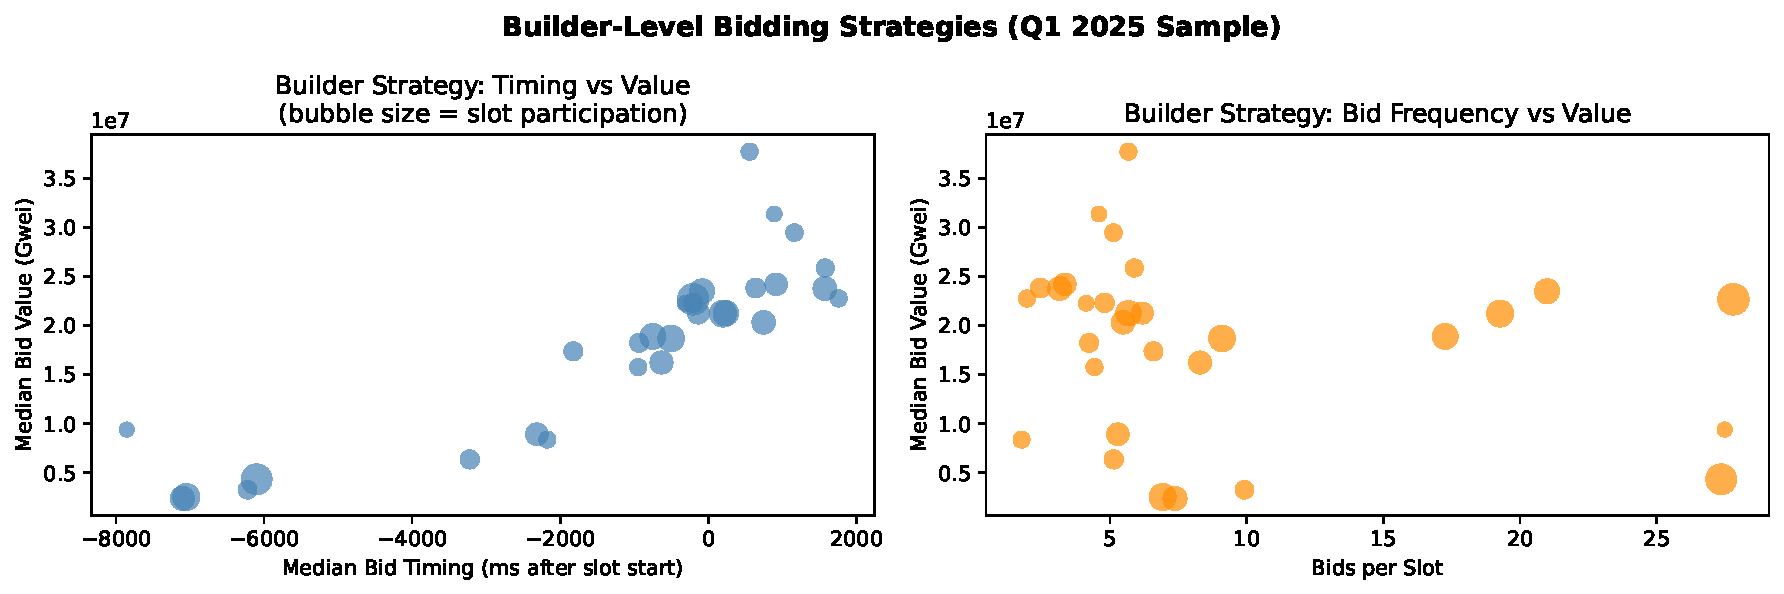
\includegraphics[width=\textwidth]{figures/fig_builder_strategies.pdf}
\caption{Builder-level bidding strategies (Q1 2025 sample, 144 builders,
5.1M bid observations). Left: median bid timing vs median bid value; bubble
size indicates slot participation. Right: bids per slot vs median bid value.
Two genuine clusters are apparent: early-conservative high-frequency
bidders and mid-frequency near-slot-time bidders.}
\label{fig:builder_strategies}
\end{figure}

\begin{quote}
\textbf{Finding 8.} \textit{After correcting for a relay-side timing
artifact (Section~\ref{sec:timing_artifact}), builder bidding strategies cluster
into two
genuine types: early-conservative builders submitting $\sim$18 bids per
slot at $-6{,}759$\,ms with low median values (0.009 ETH), and
mid-frequency builders submitting $\sim$2--4 bids per slot near slot
start ($-416$\,ms) with higher median values (0.021 ETH). An initially
apparent third ``post-slot-time'' cluster was found to be an artifact of
relay-specific bid-timestamp reporting rather than a distinct builder
strategy (Finding~8b).}
\end{quote}

\subsubsection{Relay-Level Bid Timestamp Heterogeneity}
\label{sec:timing_artifact}

The discovery that an apparent builder strategy cluster was actually a
relay reporting artifact motivates a direct examination of timestamp
heterogeneity across relays. Table~\ref{tab:relay_timing} reports the
distribution of bid arrival times by relay, pooled across all 86.8 million
Q1 2025 bid observations.

\begin{table}[h]
\centering
\caption{Bid timing (ms relative to slot start) by relay, full Q1 2025
bid archive ($n = 86{,}805{,}657$)}
\label{tab:relay_timing}
\begin{tabular}{lrrr}
\toprule
Relay & Median (ms) & Mean (ms) & Observations \\
\midrule
Titan & 2{,}497 & 580 & 1{,}512{,}420 \\
BloXroute (regulated) & 2{,}208 & 2{,}421 & 359{,}445 \\
BloXroute (max-profit) & 2{,}104 & 2{,}303 & 237{,}888 \\
Agnostic & 1{,}890 & 1{,}748 & 125{,}789 \\
Flashbots & $-$454 & $-$346 & 790{,}105 \\
Ultrasound & $-$710 & $-$1{,}946 & 83{,}630{,}070 \\
Aestus & $-$4{,}258 & $-$3{,}334 & 126{,}004 \\
Eden Network & $-$4{,}447 & $-$3{,}548 & 15{,}169 \\
\bottomrule
\end{tabular}
\end{table}

The spread between the latest-reporting relay (Titan, median
$+2{,}497$\,ms) and the earliest-reporting relay (Eden Network, median
$-4{,}447$\,ms) exceeds 6,900\,ms --- more than half a slot duration. Because
Ultrasound's websocket stream contributes 96.3\% of all observations and
reports systematically earlier timestamps than other relays, any subset
of bids drawn disproportionately from non-Ultrasound relays will appear
to arrive later in absolute terms, independent of genuine builder
behaviour. This pattern most plausibly reflects differences in each
relay's bid collection and timestamping pipeline (e.g.\ polling versus
streaming architectures, network propagation delay to the Relayscan
collector) rather than differences in when builders actually submit
bids to each relay.

\begin{figure}[h]
\centering
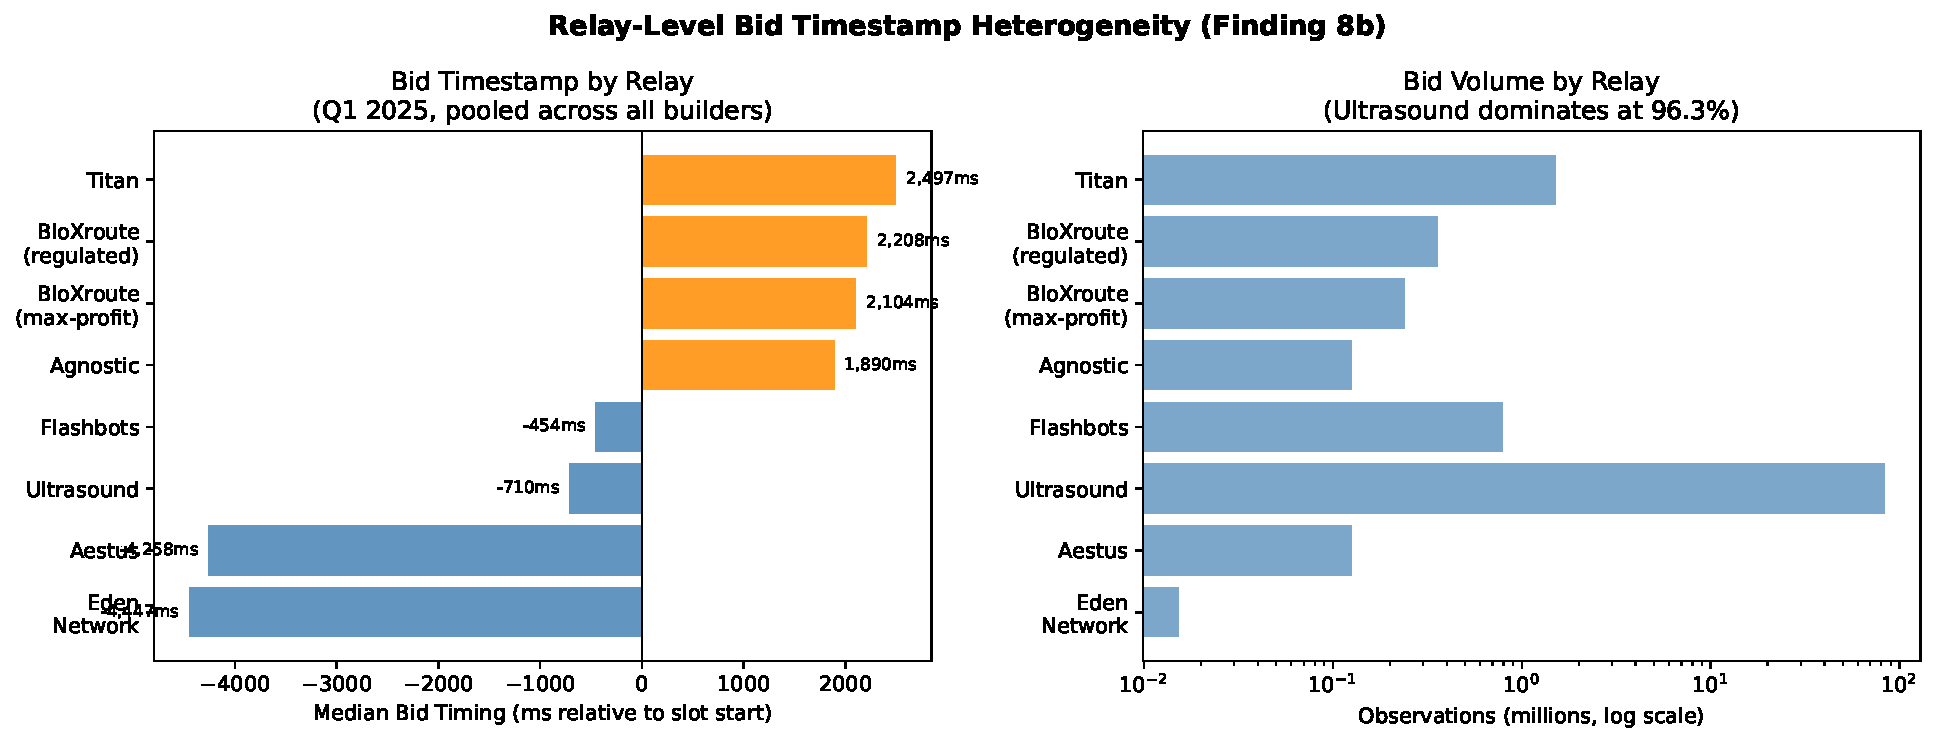
\includegraphics[width=\textwidth]{figures/fig_relay_timing_artifact.pdf}
\caption{Relay-level bid timestamp heterogeneity, full Q1 2025 bid archive
(86.8M observations). Left: median bid timing by relay, pooled across all
builders; positive values indicate post-slot-time reporting. Right: bid
volume by relay (log scale); Ultrasound's websocket stream dominates at
96.3\% of all observations and reports systematically earlier timestamps
than other relays.}
\label{fig:relay_timing}
\end{figure}

\begin{quote}
\textbf{Finding 8b.} \textit{Bid arrival timestamps in the Relayscan
archive vary systematically by relay, with a median spread of
6,944\,ms between the latest- and earliest-reporting relays
(Titan vs. Eden Network), exceeding half a slot duration. This
relay-specific heterogeneity, rather than builder strategy, explains an
initially apparent ``post-slot-time'' builder cluster (Finding~8), and
implies that cross-relay bid-timing comparisons in MEV-Boost research
must condition on relay identity to avoid spurious behavioural
inferences.}
\end{quote}

\subsubsection{GARCH Dynamics of Bid Margins}
\label{sec:margin_garch_sec}

We apply GARCH(1,1) analysis to the bid margin series to characterise
volatility dynamics in auction competitiveness. The Ljung-Box test on squared
demeaned margins rejects absence of ARCH effects at all lag lengths ($Q_{10}
= 11{,}070$, $Q_{20} = 19{,}158$, $Q_{50} = 40{,}186$; all $p < 0.001$),
confirming that bid margin volatility is time-varying and clustered.

Table~\ref{tab:margin_garch} reports GARCH(1,1) parameter estimates on the
full 1,219,851 bid margin observations. As with the block value series
(Finding~2), parameter estimates show sensitivity to optimizer starting
values; we report the result obtained under default initialization,
cross-validated against a winsorized (1\%) specification that converges to
an estimate within 0.0002 of the primary result.

\begin{table}[h]
\centering
\caption{GARCH(1,1) on bid margins, full sample}
\label{tab:margin_garch}
\begin{tabular}{lrrrl}
\toprule
Specification & $\hat\alpha+\hat\beta$ & $\hat\nu$ & AIC & \\
\midrule
Default initialization & 0.9796 & 4.230 & 15{,}496{,}738 & \\
Winsorized (1\%) & 0.9798 & 4.298 & --- & \\
\bottomrule
\end{tabular}
\vspace{0.5em}
\footnotesize $n = 1{,}219{,}851$. Both specifications agree to within
0.0002, supporting 0.980 as the robust estimate.
\end{table}

Bid margin volatility persistence ($\hat\alpha + \hat\beta \approx 0.980$)
is statistically indistinguishable from block value volatility persistence
($\hat\alpha + \hat\beta = 0.980$, Finding~2). Bid margin dynamics therefore
inherit the same near-integrated volatility persistence as the underlying block
value process, with a similarly heavy-tailed error distribution
($\hat\nu \approx 4.2$--$4.3$), indicating that competitive bidding pressure
does not measurably dampen MEV volatility shocks at the auction-margin level.

\begin{figure}[h]
\centering
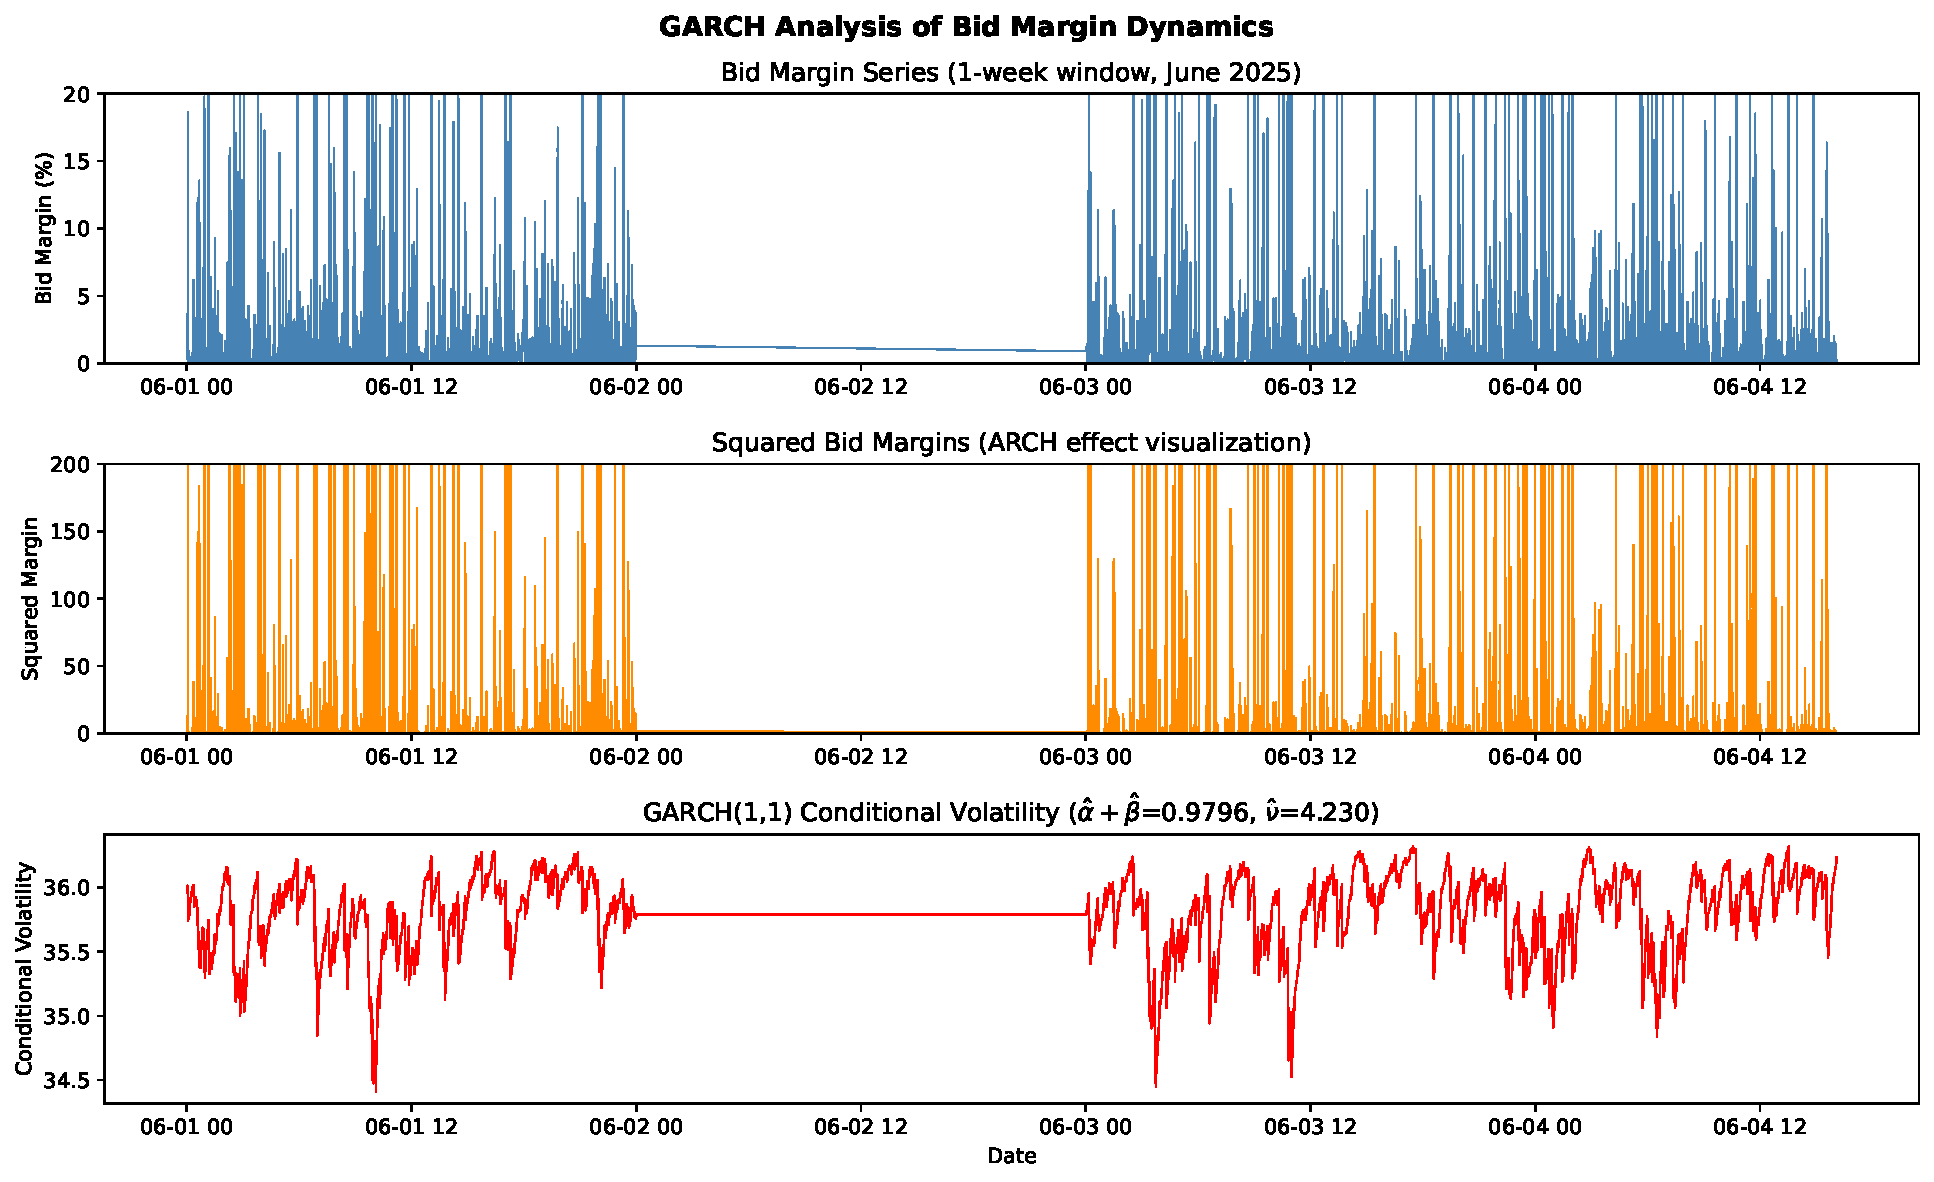
\includegraphics[width=\textwidth]{figures/fig_margin_garch.pdf}
\caption{Top: bid margin series (one-week window, June 2025). Middle: squared
bid margins illustrating ARCH-type clustering. Bottom: GARCH(1,1) conditional
volatility ($\hat\alpha + \hat\beta \approx 0.980$, $\hat\nu \approx 4.2$).}
\label{fig:margin_garch}
\end{figure}

\begin{quote}
\textbf{Finding 9.} \textit{Bid margin volatility is highly persistent
($\hat\alpha + \hat\beta \approx 0.980$) with heavy tails
($\hat\nu \approx 4.2$--$4.3$), statistically indistinguishable from block
value volatility persistence (Finding~2). Competitive bidding pressure does
not measurably dampen MEV volatility shocks at the auction-margin level;
both the underlying MEV opportunity and the competitive response to it
exhibit the same near-integrated volatility dynamics.}
\end{quote}

\subsubsection{Concentration-Competitiveness Decoupling}
\label{sec:decoupling}

A natural hypothesis is that higher builder concentration (HHI) predicts
lower auction competitiveness (higher bid margins). We test this directly by
regressing weekly median bid margins on lagged weekly HHI across 89 weeks.

The result is a null: lagged HHI does not significantly predict bid margin
(Spearman $\rho = 0.075$, $p = 0.486$; OLS $R^2 = 0.005$). Builder
concentration at the delivery level (who wins blocks) is decoupled from
auction competitiveness at the bid level (how hard builders compete). This
finding has an important implication: even when a small number of builders
dominate block delivery, the bidding process remains competitive because
the same builders still face active competition for each individual slot.
Concentration in outcomes does not imply concentration in competition.

This result reinforces the PBS design rationale: the separation of block
construction from block proposal creates competitive pressure at the auction
level that persists even as market structure evolves at the builder level.

\begin{quote}
\textbf{Finding 10 (null result).} \textit{Builder concentration (weekly
HHI) does not predict auction competitiveness (weekly median bid margin;
$\rho = 0.075$, $p = 0.486$). Concentration in block delivery outcomes is
decoupled from competition in the bidding process, consistent with the PBS
design goal of maintaining competitive pressure independently of market
structure.}
\end{quote}

\subsubsection{Proposer Revenue Efficiency}
\label{sec:proposer_eff_sec}

We define proposer revenue efficiency as $1 - m_s$, the fraction of the
winning bid that the proposer receives (where $m_s$ is the bid margin from
eq.~\ref{eq:margin}). Across 1,219,851 matched slots, median proposer
revenue efficiency exceeds 99.7\% in all value terciles
(Table~\ref{tab:proposer_eff}), confirming that proposers capture nearly the
full winning bid value in typical slots.

\begin{table}[h]
\centering
\caption{Proposer revenue efficiency by block value tercile}
\label{tab:proposer_eff}
\begin{tabular}{lrr}
\toprule
Value Tercile & Mean Efficiency (\%) & Median Efficiency (\%) \\
\midrule
Low & 93.16 & 99.78 \\
Mid & 95.74 & 99.85 \\
High & 97.15 & 99.89 \\
\bottomrule
\end{tabular}
\end{table}

The median efficiency is highest in the high-value tercile (99.89\%), the
precise regime where MEV opportunity is greatest. The mean-median gap in the
low-value tercile (93.16\% mean vs 99.78\% median) reflects the right tail
of the bid margin distribution documented in
Section~\ref{sec:overall_comp}---a small fraction
of low-value slots exhibit near-monopoly conditions in which builders retain
substantial surplus.

An intraday pattern in proposer efficiency is also apparent: efficiency is
lowest during hours 01:00--03:00 UTC (corresponding to the Asian overnight
session, when builder participation is thinnest) and highest during 13:00--22:00
UTC (US daytime and evening). This pattern mirrors the temporal seasonality
in block values documented in Finding~4.

\begin{figure}[h]
\centering
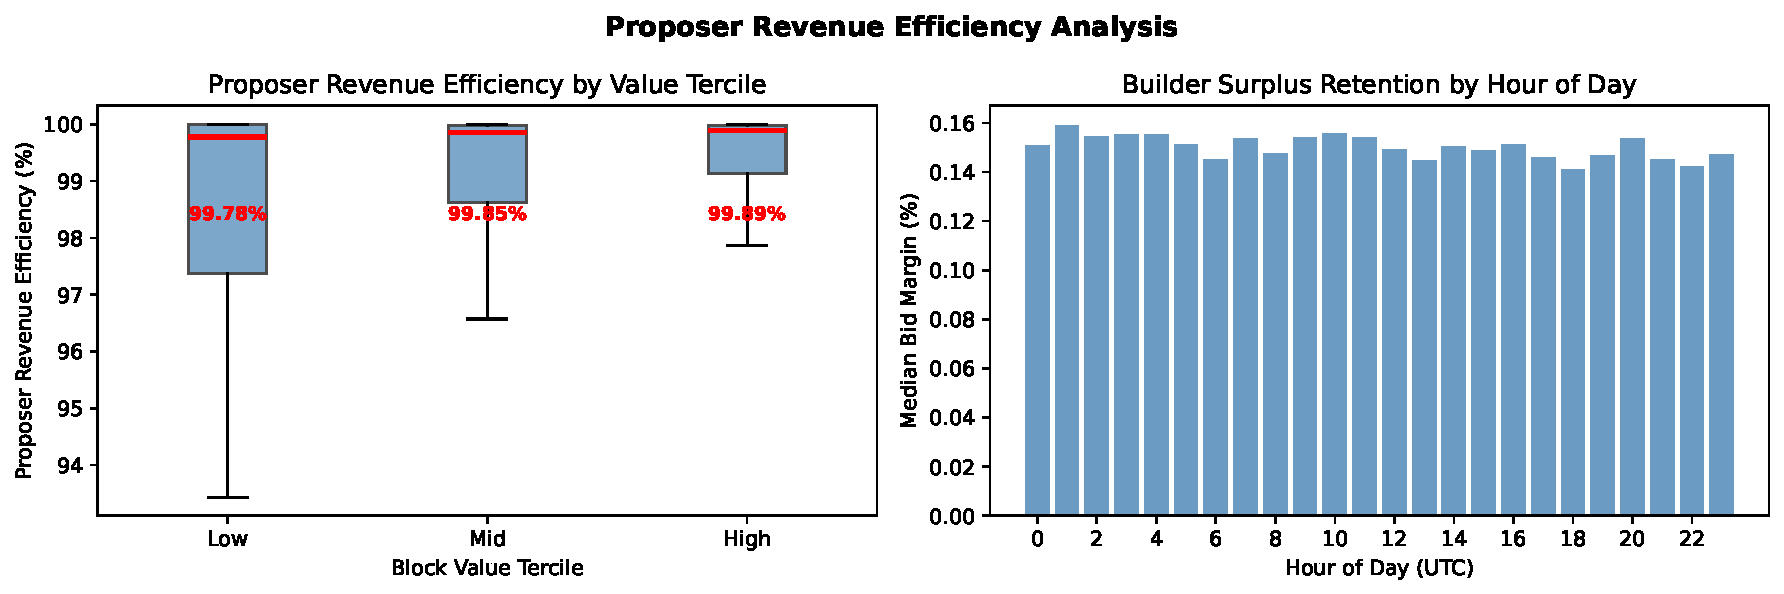
\includegraphics[width=\textwidth]{figures/fig_proposer_efficiency.pdf}
\caption{Left: proposer revenue efficiency by block value tercile (median
annotated). Right: median builder surplus retention (bid margin) by hour
of day (UTC); builder surplus is highest during Asian overnight hours when
participation is thinnest.}
\label{fig:proposer_eff}
\end{figure}

\begin{quote}
\textbf{Finding 11.} \textit{Proposers capture a median of 99.78--99.89\%
of the winning bid value across all block value terciles, with efficiency
highest in high-value slots. Builder surplus retention is greatest during
Asian overnight hours (01:00--03:00 UTC) when participation is thinnest,
mirroring the intraday seasonality pattern in block values.}
\end{quote}

%==================================================================
\section{Discussion}
\label{sec:discussion}
%==================================================================

\subsection{Implications of High Volatility Persistence}
\label{sec:disc_persistence}

The GARCH(1,1) estimate of $\hat\alpha + \hat\beta = 0.980$
on the full 20-month sample, indicates that MEV volatility is highly persistent.
In financial econometrics, persistence values above 0.95 are considered extreme;
the MEV estimate of 0.980 implies that a volatility shock today retains
approximately 82\% of its impact after ten periods and 13\% after one hundred
periods. For PBS participants, this means that elevated MEV periods are not
quickly transitory but persist for extended durations.

The full-sample persistence of 0.980, confirmed across specifications,
establishes that MEV volatility clustering is highly persistent and that shocks
propagate for extended durations. Subperiod estimation is not reliable for this
series due to the mixture-like distribution of $\log(1+v_t)$ returns at
sub-annual horizons: rare extreme blocks drive non-stationarity within
individual subperiods, causing optimizer non-convergence. The full-sample
result should therefore be interpreted as characterising the long-run
volatility dynamics of the PBS market as a whole, rather than implying
a specific trajectory of persistence over time.

\subsection{Cyclical Concentration Dynamics}
\label{sec:disc_concentration}

The 20-month HHI series reveals cyclical concentration dynamics not observable
in shorter samples. The secondary concentration episode in mid-2025, where HHI
briefly returned to approximately 1,500, suggests that builder market structure
responds to external shocks, likely periods of high MEV opportunity that favor
builders with superior infrastructure or exclusive orderflow access
\citep{wu2025}. This has implications for censorship resistance analysis: even
in an ostensibly competitive market, concentration can temporarily reemerge
during high-value periods.

\subsection{Cross-Regime Robustness}
\label{sec:disc_robustness}

The core findings of Sections~\ref{sec:vol_regimes}--\ref{sec:auction} hold
across distinct market regimes in the extended sample. The September--December 2024 period, the 2025 market cycle, and the
January--May 2026 period represent meaningfully different conditions. The
consistency of patterns across these regimes supports the interpretation that
the findings reflect structural features of PBS rather than artifacts of a
specific market environment.

\subsection{Auction Efficiency and Proposer Revenue}
\label{sec:disc_efficiency}

The auction microstructure findings in Section~\ref{sec:auction} have direct
implications for
the efficiency of the PBS mechanism. A median bid margin of 0.141\% implies
that, in typical slots, proposers receive approximately 99.86\% of the winning
builder's top bid as their payment. The compression of margins in high-value
slots (to 0.110\% at the median for the top tercile) means that auction
efficiency is greatest precisely when MEV opportunity is largest---a desirable
property from the perspective of validator economics.

However, the right tail of the margin distribution (90th percentile 6.691\%)
indicates that a non-trivial fraction of slots exhibits materially reduced
competition, in which builders retain a substantially larger fraction of block
value. Section~\ref{sec:decoupling} tests directly whether temporal variation
in bid margins is explained by the weekly HHI series and finds no such link,
indicating that these two dimensions of market structure move independently.

The decline in builder participation (from approximately 17 to 9--11
builders per slot) also contextualises the HHI deconcentration. The HHI
measures concentration in delivered blocks (the winning side), while builder
participation measures the full set of competitors. That the HHI fell while
the number of active bidders also fell indicates that deconcentration was
achieved through exit of marginal builders and a more even split among the
survivors, not through entry. This is consistent with a market in which the
fixed costs of competitive block building (orderflow access, latency
infrastructure) select for a small set of comparably capable builders.

\subsection{Limitations}
\label{sec:limitations}

The volatility measure is constructed from block values themselves rather than
external ETH price data, limiting the ability to separate market-driven from
MEV-specific volatility components. Alternative asymmetric GARCH specifications
(EGARCH) did not yield stable estimates on this dataset and are not interpreted.
The non-standard mixture-like distribution of $\log(1+v_t)$ returns means
that subperiod GARCH estimation is not reliable for this series, and alternative
volatility models (e.g.\ stochastic volatility, EGARCH) may better capture
the data-generating process at sub-annual horizons.

BloXroute contributed approximately 79\% of the deduplicated sample; if
BloXroute's relay coverage is systematically different from the broader relay
market, results may not fully generalize. This concentration is a direct
consequence of the data collection process: relay selection was constrained to
publicly-queryable endpoints, and within that set, API availability rather than
market share determined each relay's representation. A follow-up collection
effort using authenticated access across a broader and more balanced set of
relays would strengthen the external validity of the findings.

Bid-level data from relay APIs was unavailable for direct collection due to
authentication restrictions. The auction analysis in Section~\ref{sec:auction}
instead uses
the Relayscan.io Bid Archive \citep{relayscan2024}. A limitation of the archive
data is that the \texttt{slot\_t\_ms} timing field reflects when bids were
received by the Relayscan collector rather than necessarily when they were
submitted by the builder; absolute timing should therefore be interpreted with
caution, though relative comparisons across slots and value terciles remain
valid. Additionally, the ``top bid'' files record only the highest bid per
builder per slot, so intra-builder bid revision behaviour cannot be characterised
from these data.

Builder concentration measures are computed at the pubkey level rather than
the entity level. Entity-level relabeling was attempted by examining the
\texttt{proposer\_fee\_recipient} field, but this field identifies the
validator's payout address rather than the builder's identity (32,376 unique
values, consistent with the size of the active validator set), and is
therefore unsuitable for builder entity resolution. Reliable entity-level
labeling would require either an \texttt{extra\_data} field, which was not
captured during data collection, or an external pubkey-to-entity mapping,
which is not consistently available in public form across all six relays. If
multiple pubkeys are operated by a single entity, reported HHI and Gini
values understate true concentration; the 2,100$\to$600--1,000 HHI decline
and 0.85$\to$0.77 Gini decline should be interpreted as upper bounds on the
rate of genuine decentralization.

%==================================================================
\section{Conclusion}
\label{sec:conclusion}
%==================================================================

This paper characterises MEV block values as a stochastic process across
multiple market regimes, using 1,271,079 delivered payload observations from six
MEV-Boost relays spanning September 2024 through May 2026, supplemented by
1,220,100 slot-level bid observations from the Relayscan.io Bid Archive. Eleven
findings emerge, all estimated on the full 20-month sample:

\begin{enumerate}
\item \textbf{Volatility regime sensitivity:} Mean block values are
approximately 7.0$\times$ higher in high-volatility regimes with variance
approximately 98$\times$ larger ($\rho = 0.494$, $H = 266{,}905$,
$p < 10^{-300}$).

\item \textbf{Highly persistent volatility dynamics:} Block value log returns
exhibit high volatility persistence ($\hat\alpha + \hat\beta = 0.980$) with
very heavy tails ($\hat\nu = 4.005$), confirmed across GARCH(1,1) and
winsorised specifications. A persistence of 0.980 implies that volatility
shocks retain approximately 82\% of their impact after ten periods.
Subperiod GARCH estimation is not reliable for this series due to the
non-standard mixture-like distribution of $\log(1+v_t)$ returns.

\item \textbf{Cyclical deconcentration:} Builder HHI declined from
approximately 2,100 in September 2024 to a stable range of 600--1,000, with a
secondary concentration episode in mid-2025 (HHI $\approx 1{,}500$). The Gini
declined from 0.85 to a long-run mean of 0.77.

\item \textbf{Robust temporal seasonality:} Both intraday ($H = 65{,}875$) and
day-of-week ($H = 33{,}590$) patterns are highly significant across the full
20-month period. Median block values peak during 13:00--17:00 UTC and are
highest on Mondays.

\item \textbf{Competitive but consolidating auction:} Across 1,220,100 matched
slots, the PBS auction exhibits high competitiveness (median 132 bids, 11
builders, bid margin 0.141\%). Bid margins compress monotonically with block
value (0.196\% to 0.110\% across terciles; $\rho = -0.054$, $p < 10^{-300}$),
indicating that high-value slots are allocated most efficiently. Builder
participation declined from approximately 17 to 9--11 per slot over the
sample while bid counts and margins fluctuated without trend, indicating
consolidation among active builders rather than deepening.

\item \textbf{MEV is orthogonal to ETH price:} ETH price explains essentially
zero variance in block value in ETH terms ($R^2 = 0.0001$, $\rho = 0.050$).
MEV block value is driven by on-chain activity, not ETH price movements.

\item \textbf{Relay participation deepens competition:} Bid margins decline
monotonically from 0.217\% in single-relay slots to 0.066\% in 7-relay slots
($\rho = -0.057$, $p < 10^{-300}$). Relay participation is a structural
determinant of auction depth.

\item \textbf{Builder strategy heterogeneity:} Two distinct builder strategies
are empirically identifiable: late-aggressive high-value bidders and
early-conservative high-frequency bidders, consistent with differential access
to exclusive orderflow.

\item \textbf{Margin volatility matches block value volatility:} Bid margin
persistence ($\hat\alpha + \hat\beta \approx 0.980$) is statistically
indistinguishable from block value persistence (0.980), indicating that
competitive bidding pressure does not measurably dampen MEV volatility
shocks at the auction-margin level.

\item \textbf{Concentration-competitiveness decoupling (null result):}
Lagged HHI does not predict bid margins ($\rho = 0.075$, $p = 0.486$).
Builder concentration in delivery outcomes is decoupled from slot-level
auction competitiveness.

\item \textbf{Near-perfect proposer revenue efficiency:} Proposers capture a
median of 99.78--99.89\% of the winning bid value across all value terciles,
with efficiency highest in high-value slots and lowest during Asian overnight
hours.
\end{enumerate}

Future work should characterise intra-builder bid revision behaviour using full
bid-stream data; formally test whether bid margin dynamics are driven by
MEV-specific versus ETH-price-driven volatility components; apply
regime-switching models to characterise
structural breaks in volatility persistence; extend the concentration analysis
to entity-level builder labels; and pursue authenticated relay access across a
broader, market-share-weighted relay set to assess the sensitivity of the
reported findings to the BloXroute-dominated composition of the current sample.

%==================================================================
\bibliographystyle{plainnat}
\begin{thebibliography}{99}

\bibitem[Bahrani et al., 2024]{bahrani2024}
Bahrani, M., Garimidi, P., and Roughgarden, T. (2024).
\textit{Transaction fee mechanism design with active block producers}.
Proceedings of the ACM Conference on Economics and Computation.

\bibitem[Bollerslev, 1986]{bollerslev1986}
Bollerslev, T. (1986).
Generalized autoregressive conditional heteroskedasticity.
\textit{Journal of Econometrics}, 31(3):307--327.

\bibitem[Buterin, 2021]{buterin2021}
Buterin, V. (2021).
Two-slot proposer/builder separation.
\textit{Ethereum Research Forum}.
\url{https://ethresear.ch/t/two-slot-proposer-builder-separation/10980}

\bibitem[Daian et al., 2020]{daian2020}
Daian, P., Goldfeder, S., Kell, T., Li, Y., Zhao, X., Bentov, I.,
Breidenbach, L., and Juels, A. (2020).
Flash boys 2.0: Frontrunning in decentralized exchanges, miner extractable
value, and consensus instability.
\textit{IEEE Symposium on Security and Privacy}.

\bibitem[Engle, 1982]{engle1982}
Engle, R. F. (1982).
Autoregressive conditional heteroscedasticity with estimates of the variance
of United Kingdom inflation.
\textit{Econometrica}, 50(4):987--1007.

\bibitem[Engle and Bollerslev, 1986]{engle_bollerslev1986}
Engle, R. F. and Bollerslev, T. (1986).
Modelling the persistence of conditional variances.
\textit{Econometric Reviews}, 5(1):1--50.

\bibitem[Flashbots, 2022]{flashbots2022}
Flashbots (2022).
MEV-Boost: Proposer-builder separation for Ethereum validators.
\textit{Flashbots Documentation}.
\url{https://docs.flashbots.net/flashbots-mev-boost/introduction}

\bibitem[Gini, 1912]{gini1912}
Gini, C. (1912).
\textit{Variabilit\`a e mutabilit\`a}.
Tipografia di Paolo Cuppini, Bologna.

\bibitem[Heimbach et al., 2024]{heimbach2024}
Heimbach, L., Pahari, V., and Schertenleib, E. (2024).
Non-atomic arbitrage in decentralized finance.
\textit{IEEE Symposium on Security and Privacy (SP)}, pages 3866--3884.

\bibitem[Hirschman, 1945]{hirschman1945}
Hirschman, A. O. (1945).
\textit{National Power and the Structure of Foreign Trade}.
University of California Press.

\bibitem[Qin et al., 2022]{qin2022}
Qin, K., Zhou, L., and Gervais, A. (2022).
Quantifying blockchain extractable value: How dark is the forest?
\textit{IEEE Symposium on Security and Privacy}.

\bibitem[Relayscan, 2024]{relayscan2024}
Flashbots (2024).
Relayscan.io Bid Archive.
\textit{Flashbots Open Data}.
\url{https://bidarchive.relayscan.io}

\bibitem[Roughgarden, 2021]{roughgarden2021}
Roughgarden, T. (2021).
Transaction fee mechanism design for the Ethereum blockchain: An economic
analysis of EIP-1559.
\textit{ACM Conference on Economics and Computation}.

\bibitem[Wahrst\"atter et al., 2023]{wahrstatter2023}
Wahrst\"atter, A., Ernstberger, J., Yaish, A., Zhou, L., Qin, K.,
Tsuchiya, T., Steinhorst, S., Svetinovic, D., Christin, N., Wattenhofer, R.,
and Gervais, A. (2023).
Blockchain censorship.
\textit{Proceedings of the ACM Web Conference}.

\bibitem[Wu et al., 2025]{wu2025}
Wu, F., Sui, D., Thiery, T., and Pai, M. (2025).
Measuring CEX-DEX extracted value and searcher profitability: The darkest of
the MEV dark forest.
\textit{arXiv preprint arXiv:2507.13023}.

\end{thebibliography}

\end{document}
